%%%%%%%%%%%%%%%%%%%%%%%%%%%%%%%%%%%%%%%%%%%%%%%%%%%%%%%%%%%%%%%%%%%%%%%%%%%%%%%%%%%%%%%%%%%%%%%%%%%%%%%%%%%%%%%%%%%%%%%%%%%%%%%%%%%%%%%%%%%%%%%%%%%%%%%%%%%
% This is just an example/guide for you to refer to when submitting manuscripts to Frontiers, it is not mandatory to use Frontiers .cls files nor frontiers.tex  %
% This will only generate the Manuscript, the final article will be typeset by Frontiers after acceptance.   
%                                              %
%                                                                                                                                                         %
% When submitting your files, remember to upload this *tex file, the pdf generated with it, the *bib file (if bibliography is not within the *tex) and all the figures.
%%%%%%%%%%%%%%%%%%%%%%%%%%%%%%%%%%%%%%%%%%%%%%%%%%%%%%%%%%%%%%%%%%%%%%%%%%%%%%%%%%%%%%%%%%%%%%%%%%%%%%%%%%%%%%%%%%%%%%%%%%%%%%%%%%%%%%%%%%%%%%%%%%%%%%%%%%%

%%% Version 3.4 Generated 2018/06/15 %%%
%%% You will need to have the following packages installed: datetime, fmtcount, etoolbox, fcprefix, which are normally inlcuded in WinEdt. %%%
%%% In http://www.ctan.org/ you can find the packages and how to install them, if necessary. %%%
%%%  NB logo1.jpg is required in the path in order to correctly compile front page header %%%

\documentclass[utf8]{frontiersSCNS} % for Science, Engineering and Humanities and Social Sciences articles
%\documentclass[utf8]{frontiersHLTH} % for Health articles
%\documentclass[utf8]{frontiersFPHY} % for Physics and Applied Mathematics and Statistics articles
%\setcitestyle{square} % for Physics and Applied Mathematics and Statistics articles

\usepackage{url,lineno,microtype,subcaption}

\usepackage[onehalfspacing]{setspace}

\usepackage{braket}

\usepackage[colorlinks]{hyperref}
\hypersetup{citecolor={blue}}
\hypersetup{urlcolor={blue}}
\hypersetup{linkcolor={blue}}

\usepackage{lmodern}
\usepackage{amsmath}
\usepackage[T1]{fontenc}
\usepackage[utf8]{inputenc}


\linenumbers
\usepackage{xcolor}
\usepackage{amsmath}
\usepackage{amstext}
\usepackage{graphicx}
\usepackage{color}				
\usepackage{multirow}	
\usepackage{setspace}

% Leave a blank line between paragraphs instead of using \\


\def\keyFont{\fontsize{8}{11}\helveticabold }
\def\firstAuthorLast{Sample {et~al.}} %use et al only if is more than 1 author
\def\Authors{Eliezer Gurarie\,$^{1,2,*}$, 
	Sriya Potluri\,$^1$, 
	G.~Christopher Cosner\,$^3$,
	R.~Stephen Cantrell\,$^3$,
	William F.~Fagan\,$^1$
}
% Affiliations should be keyed to the author's name with superscript numbers and be listed as follows: Laboratory, Institute, Department, Organization, City, State abbreviation (USA, Canada, Australia), and Country (without detailed address information such as city zip codes or street names).
% If one of the authors has a change of address, list the new address below the correspondence details using a superscript symbol and use the same symbol to indicate the author in the author list.
\def\Address{$^{1}$Department of Biology, University of Maryland, College Park, MD 20742, USA.\\
	$^{2}$Department of Environmental and Forest Biology, SUNY College of Environmental Science and Forestry, Syracyse, NY 13210, USA.\\
	$^{3}$Department of Mathematics, The University of Miami, Coral Gables, FL 33146, USA.
}
% The Corresponding Author should be marked with an asterisk
% Provide the exact contact address (this time including street name and city zip code) and email of the corresponding author
\def\corrAuthor{Eliezer Gurarie}
\def\corrEmail{egurarie@umd.edu}




\begin{document}
	\onecolumn
	\firstpage{1}
	
	\title[Sociality, memory and migration]{Memories of migrations past: Sociality and cognition in dynamic, seasonal environments} 
	
	\author[\firstAuthorLast ]{\Authors} %This field will be automatically populated
	\address{} %This field will be automatically populated
	\correspondance{} %This field will be automatically populated
	
	\extraAuth{}% If there are more than 1 corresponding author, comment this line and uncomment the next one.
	%\extraAuth{corresponding Author2 \\ Laboratory X2, Institute X2, Department X2, Organization X2, Street X2, City X2 , State XX2 (only USA, Canada and Australia), Zip Code2, X2 Country X2, email2@uni2.edu}
	
	
	\maketitle
	
	
	\begin{abstract}
		
	Seasonal migrations are a widespread and broadly successful strategy for animals to exploit periodic and localized resources over large spatial scales.  It remains an open and largely case-specific question whether long-distance migrations are resilient to environmental disruptions. High levels of mobility suggest an ability to shift ranges that can confer resilience. On the the other hand, a conservative, hard-wired commitment to a risky behavior can be costly if conditions change. 
	
	Mechanisms that contribute to migration include identification and responsiveness to resources, sociality, and cognitive processes spatial memory and learning.  Our goal was to explore the extent to which these factors interact not only to maintain a migratory behavior but also to provide resilience against environmental changes. We develop a relatively simple diffusion-advection model of animal movement in which an endogenous migratory behavior is modified by recent experiences via a memory process, and animals have a social swarming-like behavior over a range of spatial scales. 
	
	We found that this relatively simple framework was able to adapt to a stable, seasonal resource dynamic under a fairly broad range of parameter values. Furthermore, the model was able to acquire an adaptive migration behavior with time. However, the resilience of the process depended on all the parameters under consideration, with many complex trade-offs. For example, the spatial scale of sociality needed to be large enough to capture changes in the resource, but not so large that the acquired collective information was overly diluted.   A long-term reference memory was important for hedging against a highly stochastic process, but a higher weighting of more recent memory was needed for adapting to directional changes in resource phenology. 
	
	Our model provides a general and versatile framework for exploring the interaction of memory, movement, social and resource dynamics, even as environmental conditions globally are undergoing rapid change. 
		
				
		\tiny
		\keyFont{ \section{Keywords:} Sociality, seasonal migration, collective knowledge, diffusion-advection models, spatial memory} 
	\end{abstract}
	
\section{Introduction}
	
	Seasonal migrations are widespread among terrestrial, aquatic, avian and invertebrate species \citep{Dingle2014}. For many species, migration is an extremely successful strategy, allowing a far greater number of individuals to inhabit landscapes which might not otherwise be able to support large numbers year round \citep{Fryxell1988}. The evolutionary stability of a migratory strategy essentially relies on the fitness benefits of accessing seasonal resources, whether for energetic gain, predator avoidance, or a suitable  environment for reproduction, outweighing the energetic and survival related costs of migration \citep{Avgar2014}. 
	
	Proximate causes, drivers and mechanisms for migration vary widely across and even within species \citep{Berthold1999, Shaw2016}. Some migrants follow a ``green wave'' of spring vegetation as it flowers across altitudinal or latitudinal gradients \citep{Bischof2012, Kolzsch2015, Merkle2016}. These migrations can be considered ``tactical'', as they can occur - as an extreme simplification - purely as response to local conditions. Other migrants perform long-distance migrations in anticipation that critical resources will be available at the time of arrival at the end point of migration \citep{Abrahms2019}. This second behavior involves the greatest trade-off between the costs and benefits of accessing those highly seasonal and localized resources. This approach can be considered ``strategic'' in the sense that it is driven not by immediate cues but by an anticipation based on prior experience \citep{Bracis2017, Merkle2019, Bauer2020}. 

	While migration can be a very successful strategy, with migratory ecotypes of the same species often outnumbering non-migratory conspecifics.  Migratory caribou and reindeer \emph{Rangifer tarandus}, for example, are several orders of magnitude more abundant than non-migratory woodland, mountain and forest ecotypes \citep{FestaBianchet2011,Uboni2016}. However, the question of whether migratory animals are more or less resilient to environmental disruptions in the environment remains open and largely case-specific \citep{Moore2008, HardestyMoore2018, Xu2021}. On the one hand, migratory species may be more vulnerable as disruptions in either of the seasonal ranges or along a migratory corridor can have significant negative impacts \citep{Wilcove2008, Seebacher2015, Kauffman2021}. On the other hand, migratory species might be more resilient due to their general wide-ranging mobility \citep{Robinson2009}. The resilience of a migratory populations depends on the plasticity and adaptability of a population, which can take multiple forms, reflecting variation in \textit{where}, \textit{when} and \textit{whether} the migration occurs \citep{Gurarie2017, Xu2021}. 
	
	Cognitive processes, in particular spatial memory, have been shown to be important mechanisms for the reinforcement and maintenance of migration \citep{Merkle2019, Bauer2020}. Similarly, sociality and social learning are likely essential to maintaining migration \citep{Guttal2010, Fagan2011, Jesmer2018, Berdahl2018}.  However, the interacting role of sociality and spatial memory for the plasticity of migration and the resilience of the behavior when faced with a changing environment are generally unknown, though it has been hypothesized that the importance of these cognitive processes depend on the predictability of these resources \citep{RiotteLambert2020}. Because the scenarios underlying migration are manifold and complex, mathematical modeling may provide some insights and help clarify where, when, and under what conditions we might expect migration behavior to emerge, to be adaptive, to be maladaptive, or to collapse.

	Here, we develop a diffusion-advection model with sociality and memory to explore the resilience of a migratory population under various dynamic, seasonal resource distributions. In formulating the model, our goal was to identify the minimum set of movement and memory parameters required to generate an adaptive, migratory behavior. This includes the ability to learn to migrate from non-migratory initial conditions, simulating the release of naive animals in a seasonal environment \citep{Jesmer2018}, to lose the propensity to migrate if the resource distribution does not require it, also a commonly observed phenomenon \citep{Wilcove2008}, and to assess the resilience or fragility of a migratory population against changing resource distribution dynamics, including both stochasticity and trends in spatial and temporal distributions, mirroring the effects of climate change \citep{Park2020}.
	
	We anticipated that under many conditions a blending of \emph{tactical} (i.e.~direct response to resource availability or perception) and \emph{strategic} (i.e.~memory-driven and forward-thinking) behavior will help foragers navigate dynamic, seasonal environments. Over-reliance on either strategy should be maladaptive. We further anticipate that a shorter-term memory updating is needed to navigate trends in resource spatial distribution and temporal distribution (phenology), but that a longer-term reference memory is needed to navigate resource distributions that are stochastic \citep{Lin2021}. Similarly, we anticipated that a balance between very low sociality and extreme sociality would lead to the most resilient migratory process. 
	
\section{Methods}
~
\subsection{Memory movement model}

	In designing our study, our goal was to develop a minimal heuristic in which the following processes were explicitly modeled: (1) Random or exploratory movement, (2) attraction to resources, (3) sociality in the movements, (4) a long-term (or \emph{reference}) memory of large-scale movement behavior, and (5) a short-term (or \emph{working}) memory that updates movement behavior based on recent experience.  
	
	A diffusion-advection equation provided a computationally efficient and versatile framework for examining just such a system. We consider a population moving in one dimension in a constrained domain $D$ and distributing itself according to the following equation:
	
	\begin{equation}\label{eq_mainmodel}
		-{\frac{\partial u}{\partial t}} = -\varepsilon {\frac{\partial^2 u}{\partial x^2}} + 
		\alpha \frac{\partial}{\partial x}\left(u \frac{\partial h}{\partial x}\right) + 
		\beta \frac{\partial}{\partial x}\left(v_s(u)\right) + \frac{\partial}{\partial x}\left(u\,v_m(t)\right)
		\end{equation}
	
	\noindent where $u$ represents the population distributed in time and space. The first term is the diffusion term, capturing the fast time-scale exploration and ``random'' movements of individuals, with $\varepsilon$ is the diffusion rate.
	
	The second term represents the attraction to a dynamic resource $h$, with the proportionality of the advection to the gradient of the resource given by the parameter $\alpha$ (note, the population and resource distributions are functions of both space and time $u(x,t)$ and $h(x,t)$ - we omit the dependent variables in the notation for brevity). This is the well-studied standard chemotaxic resource-following behavior. We borrow the general notation from earlier related work expanding diffusion-advection models to incorporate non-local information \citep{Fagan2017} and behavioral switching \citep{Fagan2019}.
	
	The third term captures the collective or social advection term of the population via a non-local, density dependent function $v_s(u,x)$. If this function takes the form of a convolution around a non-local kernel $k$, i.e.~$v_s(u) = k(x) * u(x)$, and if that kernel is odd, an attractive or ``swarming'' behavior can be generated \citep{Mogilner1999}. We use the kernel analyzed by \citet{Mogilner1999}: 
	
	$$k(x) = \frac{x}{2\lambda^2} \exp(-x^2/2\lambda^2).$$ 
	
	\noindent The convolution of $u$ with this kernel has the property of pushing the population in a positive direction when $x < \braket{u}$, and in a negative direction when $x > \braket{u}$, where $\braket{u}$ is the mean location of the population. The parameter $\lambda$ is a length scale of sociality, roughly one-half the size of the swarm, and $\beta$ is a parameter that quantifies the overall strength of sociality.
	
	Finally, the last term captures the direct advection that emerges from a memory-driven migratory behavior. This term evolves with a set of parameters $\theta_y$ that slowly change each year $y \in \{0,1,2,...\}$, i.e.~the count of periods $\tau$: $y = \lfloor t/\tau \rfloor$.  The migration is specified by six parameters $\theta$: the timing of the start and duration of two anticipated seasons (e.g.~summer and winter) $t_1$, $\Delta t_1$, $t_2$, $\Delta t_2$, and the spatial coordinates of the population centroid for each season $x_1$ and $x_2$. The remembered migratory speed term is a simple step function given by:
	
	\begin{equation}
		v_m(t, \theta_y) = \begin{cases}
			0; & t > t_1  \,\, \text{and} \,\, t \leq t_1 + \Delta t_1 \\ 
			s_{12}; & t > t_1 + \Delta t_1 \,\, \text{and} \,\,  t \leq t_2 \\ 
			0; & t> t_2 \,\, \text{and} \,\, t \leq t_2 + \Delta t_2 \\ 
			s_{21}; &  t > t_2+\Delta t_2 \,\, \text{or} \,\, t \leq t_1\\ 
		\end{cases}
	\end{equation}
	
	\noindent where the migration speeds $s_{12}$ and $s_{21}$ from the respective ranges are set such that they arrive at $x_1$ at $t_1$, depart at $t = t_1 + \Delta t_1$, arrive at $x_2$ at $t = t_2$, and depart at $t_2 + \Delta t_2$. Thus, $s_{12} = (x_2-x_1)/ (t_2 - (t_1 + \Delta t_1))$ and $s_{21} = (x_1-x_2)/(t_1 - (t_2 - \tau + \Delta t_2))$. This step-like migration function is a one-dimensional version of the migration parameters estimated for individuals \citep{Gurarie2017} and populations \citep{Gurarie2019} in empirical studies.
	
	We consider these six parameters to be the known or remembered determinants of the migratory behavior, with an initial set $\theta_0$ determining the reference migration behavior. This reference migration is updated each year by the experience of the population. To perform this updating, we estimate a new set of parameters $\widehat{\theta_y}$ after each year, and combine these new parameters with the reference parameters according to the following weighted mean:
	
	\begin{equation}\label{eq_memory}
	\theta_{y+1} = \kappa^y \, \theta_o + \left(1-\kappa^y\right)\,\widehat{\theta_y} 
\end{equation}
	
	\noindent where each of the six parameters is updated according to equaton \ref{eq_memory} identically. The estimates $\widehat{\theta_y}$ are obtained via a least-squares minimization of the migration track ($m(t,\theta) = \int_0^t v_m(t',\theta_y) \, dt'$) against the spatial mean of the population process in year $y$ (i.e.~$\widehat{u}(t) = \int_X u_y(t, x) dx$). The parameter $\kappa \in (0,1)$ captures the reliance on that long-term memory. When $\kappa = 0$, all of the actionable memory is from the preceding year. When $\kappa = 1$, the actionable memory is entirely the reference memory.
	
	The model is confined to a one-dimensional bounded domain $[-\chi,\chi]$, with no flux outside of the boundaries. Formally, this no-flux condition means the following conditions must be met 
	
	$$
	\begin{cases}
		\varepsilon \frac{\partial u}{\partial x} - 		
	\alpha \left(u \frac{\partial h}{\partial x}\right) - \beta(v_x(u)) - (uv_m(t)) = 0 & \text{where}\,\, x = \chi\\
	-\varepsilon \frac{\partial u}{\partial x} - 
	\alpha \left(u \frac{\partial h}{\partial x}\right) - \beta(v_x(u)) - (uv_m(t)) = 0 & \text{where}\,\, x = -\chi
	\end{cases}
$$


	\noindent In practice, the design of our resource space (see below) and other parameterization lead 0 or near 0 values of both $h(x)$ and $u(x)$, and the simpler ${\partial u(-\chi,t)}/{\partial t} = {\partial u(\chi,t)}/{\partial t} =0$ boundary condition provides a good approximation. 
	
	As there are no birth or death processes, the total population remains fixed and constant, for convenience integrating to 1. Furthermore, the parameters remain constant throughout time, with no adaptation or mutation-selection process. Our interest is in the ability of a fixed set of movement and memory parameters to navigate an intra- and interannually dynamic, seasonal environment.
	
	
\subsection{Seasonal resource}
	
	We ran this model on a spatial domain $x \in [-100,100]$, and a periodicity $\tau = 100$ (i.e.~100 day years). We were interested in an approximately periodic resource dynamic, i.e.~one in which $h(x,t) \approx h(x, t-\tau))$. We generated two types of resource distributions. A ``non-surfable'' resource (\emph{island resource}), and weakly surfable resource (\emph{drifting resource}). Both are characterized by a peak in time and space centered at $m_x$ at $m_t$, and $-m_x$ at $\tau - m_t$ (for example, locations 30 and $-30$ at times 25 and 75, respectively). These pulses have a shared time scale of duration $s_t$ and a spatial scale of extent $s_x$, the standard deviation in the time and space dimension respectively. The island resource is simply two uncorrelated bivariate normal
	distributions 
	
	$$h(x,t) = K\,(\Phi(m_x, m_t, s_x, s_t) + \Phi(-m_x, \tau - m_t, s_x, s_t))$$ 
	
	\noindent where $\Phi$ is the bivariate Gaussian distribution function, and the normalizing constant $K$ is selected such that the average total amount of resource throughout the year is 1, i.e.~$\frac{1}{\tau} \int_T\int_X h(x,t) dx\,dt = 1$.
	
	The drifting resource differs from the island resource in that the total amount of resource at any given time $\int_X h(x,t) dx = 1$. This property is attained by distributing the resource as a re-scaled beta distribution, where the shape and scale parameters vary sinusoidally in such a way as to make the standard deviations and means match the desired values of $m_x, m_t, s_x, s_t$ (see Supplementary Materials for details). Both types of resources are illustrated in figure \ref{fig_ResourceExamples}.
	
	Within a given year, the resource is entirely symmetric: $h_y(x,t) = h_y(-x, \tau-t)$. However, in scenarios exploring climate change we allow the peaks to vary with directional trend and stochasticity according to: $m_x(y) \sim {N}(\mu_x + \gamma_x\,y, \sigma_x)$ and $m_t(y) \sim {N}(\mu_t + \gamma_t\,y, \sigma_t)$, where the $\mu$, $\gamma$ and $\sigma$ terms are the mean, slope and variance, respectively, for the location and time duration of the pulse. Thus, if $\gamma=0$ and $\sigma=0$, the conditions are constant across years and if $\gamma_x > 0$ there is a shift of the resource towards the extremes of the domain. While we did not explore phenological shifts in timing, those can readily be modeled as well. These trends model the pole-ward shift of peak resources and the earlier spring phenology occurring with a warming global climate \citep{Renner2018}. The spatial and temporal scales of the resource peak ($s_x$ and $s_t$) remain constant in all of our simulations. 
	
	\begin{figure}[t!]
		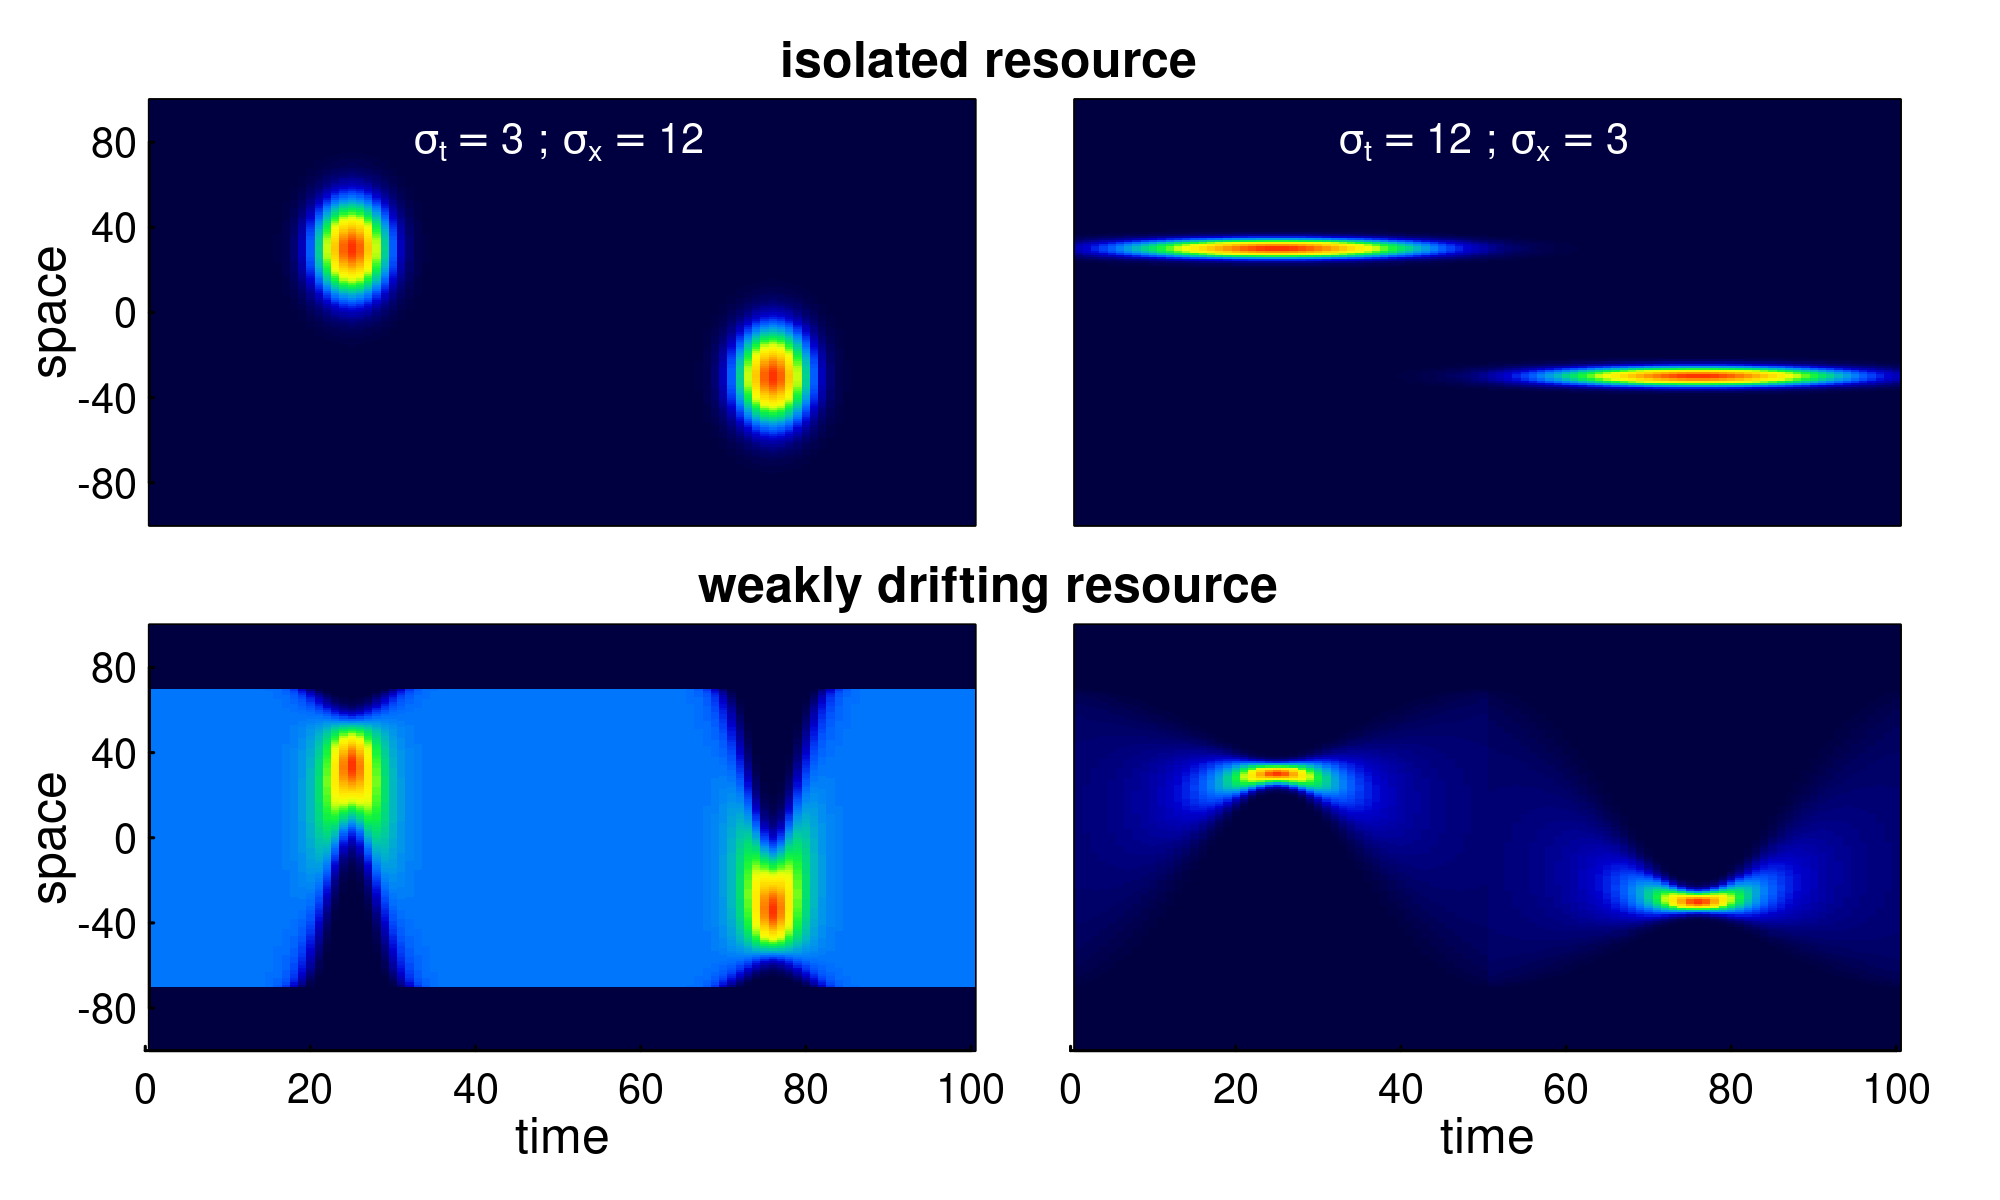
\includegraphics[width = \textwidth]{figures/ResourceExamples.png}
		
		\caption{\label{fig_ResourceExamples}  Examples of various seasonal resource distribution functions, contrasting short duration, but wide pulses ($\sigma_t = 3, \sigma_x = 12$; left panels), long duration but spatially concentrated pulses ($\sigma_t = 12, \sigma_x = 3$; right panels), and isolated resource pulses (upper panels) from the weakly drifting resource (lower panels). The total amount of resource is identical across all scenarios. In the weakly drifting resources, the total amount is constant at all times, and uniform in the middle of the phase (time = 0, 50, 100).}
	\end{figure}
	
\subsection{Metrics}
	
	The main metrics we were interested in are \emph{migration mismatch}, \emph{foraging efficiency} and \emph{adaptation to directional trends}.
	
	Migration mismatch captures the combined difference between the migration phenology and the resource phenology in time and space. Spatial mismatch $\text{MM}_x$ is the absolute difference between the migration targets and the resource peaks: $\text{MM}_x = |x_1 - m_x| + |x_2 + m_x|$. Temporal mismatch is the difference between the arrival time and the peak of the resource if arrival is post-peak, the difference between the departure time and the peak of the resource if departure is pre-peak, and 0 if the seasonal duration spans the peak, i.e.~$\text{MM}_t = max\{t_1 - m_1, m_1 - (t_1 + \Delta t_1), 0\} + max\{t_2 - m_2, m_2 - (t_2 + \Delta t_2), 0\}$. Thus, the total mismatch is the sum of these: $\text{TM} = \text{MM}_x + \text{MM}_t$. A mismatch of less than 1 is essentially perfect, a mismatch of 1-5 we consider excellent, and beyond 50 the system can be said to have failed to keep track of the resource dynamics.
	
	To quantify the foraging efficiency, i.e.~the organisms' ability to track the distribution of the resources over space and time, we use a continuous form of the Bhattacharyya coefficient \citep{Bhattacharyya1943} which quantifies the similarity between two distributions. We compute this coefficient at every time point in a given year, and take the mean across the equilibrium year to determine foraging efficiency (FE). Thus, the foraging efficiency index is:
	
	$$\text{FE} = \frac{1}{\tau} \int_{0}^\tau \int_{-\chi}^{\chi} \sqrt{u(x,t) \, h(x,t)} \,\, dx\,dt$$
	
	\noindent where the spatial integral is taken over the domain. This metric is constrained to be between 0 and 1.
	
	For simulations with a constant resource, we ran the model until a quasi-equilibrium (stationary) state was achieved, i.e.~where the Bhattacharya index of the population distribution across subsequent years reached a value of $0.99999$. Once stationarity was attained, we computed the migration mismatch and foraging efficiency metrics, as well as the number of years required to reach stationarity.
	
	For numerical runs with climate change, we first run a simulation with a given parameter set until stationarity, as above, and then begin shifting the location of the resource poleward with a slow, moderate or rapid trend ($\gamma_x = 0.25, 0.5$ and 1, respectively), and / or by adding stochasticity (spatial standard deviation 3, 6, 9 or 12). For stochasticity analyses, we compare foraging efficiency across a range of the reference memory parameter $\kappa$.  For analyses that included directional trends, with or without stochasticity, we quantified the ability of the system to keep track of climate change with a \emph{spatial adaptation} (SA) index. This index is the ratio of the slope of the memory-based migration location over time, i.e.~$\text{SA} = \widehat{\gamma}/\gamma_x$  where the adaptation slope estimate is the regression coefficient of the spatial coordinate of the migration against time (i.e.~$m_{x,i} = \widehat{\gamma_x} i + m_{x,0}$, where $i$ is the year), and $\gamma_x$ is the rate of drift of the resource peak (table \ref{table_definitions}). An SA equal to 1 suggests that the process is keeping up with climate change, an SA of 0 indicates that the process is not responding at all to climate change.  Values greater than 1 (super-adaptation) are possible, as are values less than 1, which correspond to a loss of migration behavior. All movement model parameters, resource parameters, and metrics are summarized in table \ref{table_definitions}. \\
	
\subsection{Simulation studies}
	
	We explored this model using numerical differencing of a system of ordinary differential equations (ODE's) approximating the PDE in equation \ref{eq_mainmodel} with the Runge-Kutte algorithm using the \texttt{deSolve} \citep{Soetaert2010} and \texttt{ReacTran} \citep{Soetaert2012} packages in R. We additionally used the \texttt{nlsLM} function in package \texttt{minpack.LM} \citep{minpack.lm} for robust and fast annual estimation of the migration parameters. The complete code is available as an R package (\texttt{memorymigration}) available on GitHub at \url{https://github.com/EliGurarie/memorymigration} and as an interactive Shiny application at \url{https://spot3512.shinyapps.io/memorymigrationshinyapp/}.
	
	We assessed a wide range of parameter values and resource geometries and dynamics with the goal of answering the four main questions: (1) Can this model adapt to a discrete shift in peak resource location and timing?  What is the relative role of memory and sociality for adaptation? (2) Can this model acquire a migratory behavior from a non-migratory initial condition? (3) What is the role of a reference memory for dealing with stochastic resource dynamics? (4) Can this model adapt when the resource peaks shifts in space?  Details of parameter combinations and reported metrics are provided in respective results sections. 
	
	\begin{table}[b!]
		\caption{\label{table_definitions} Table of parameters, variables and metrics.}
		
		\centering
		\begin{tabular}{ll|l}
			\hline\hline
			\multicolumn{3}{l}{\textbf{Memory migration model}}\\ 
			& $\varepsilon$ & Diffusion \\ 
			& $\alpha$ & Strength of resource following \\ 
			& $\beta$ & Strength of sociality \\ 
			& $\lambda$ & Spatial scale of sociality \\ 
			& $\kappa$ & Initial weighting of reference versus working memory \\ 
			& $x_1$, $x_2$ & location of population centroids in summer and winter \\ 
			& $t_1$, $\Delta t_1$ & start and duration of summer season \\ 
			& $t_2$, $\Delta t_2$ & start and duration of winter season \\ 
			&& (long-term) memory vs. working (short-term) memory \\ 
			\multicolumn{3}{l}{\textbf{Resource dynamics}} \\ 
			& $\tau$ & duration of period (year) \\ 
			& $m_x$, $-m_x$ & spatial coordinate of resource peak for summer and winter \\ 
			& $m_t$, $\tau - m_t$ & timing of resource peak for the summer and winter \\ 
			& $\sigma_x$, $\sigma_t$ & time duration and spatial scale of resource pulse \\ 
			& $\gamma_x$, $\gamma_t$ & rate of change of peak location and timing of resource \\ 
			& $\psi_x$, $\psi_t$ & standard deviation of peak location and timing \\ 
			\multicolumn{3}{l}{\textbf{Metrics}}\\ 
			& $\text{MM}_x$ & spatial migration mismatch \\ 
			& $\text{MM}_t$ & temporal migration mismatch \\ 
			& $\text{TM}$ & total mismatch \\ 
			& $\text{FE}$ & foraging efficiency \\ 
			& $\text{SA}$ & spatial adaptation index \\ 
			\hline\hline
		\end{tabular}
	\end{table}
	
\section{Results}
	
	\begin{figure}
		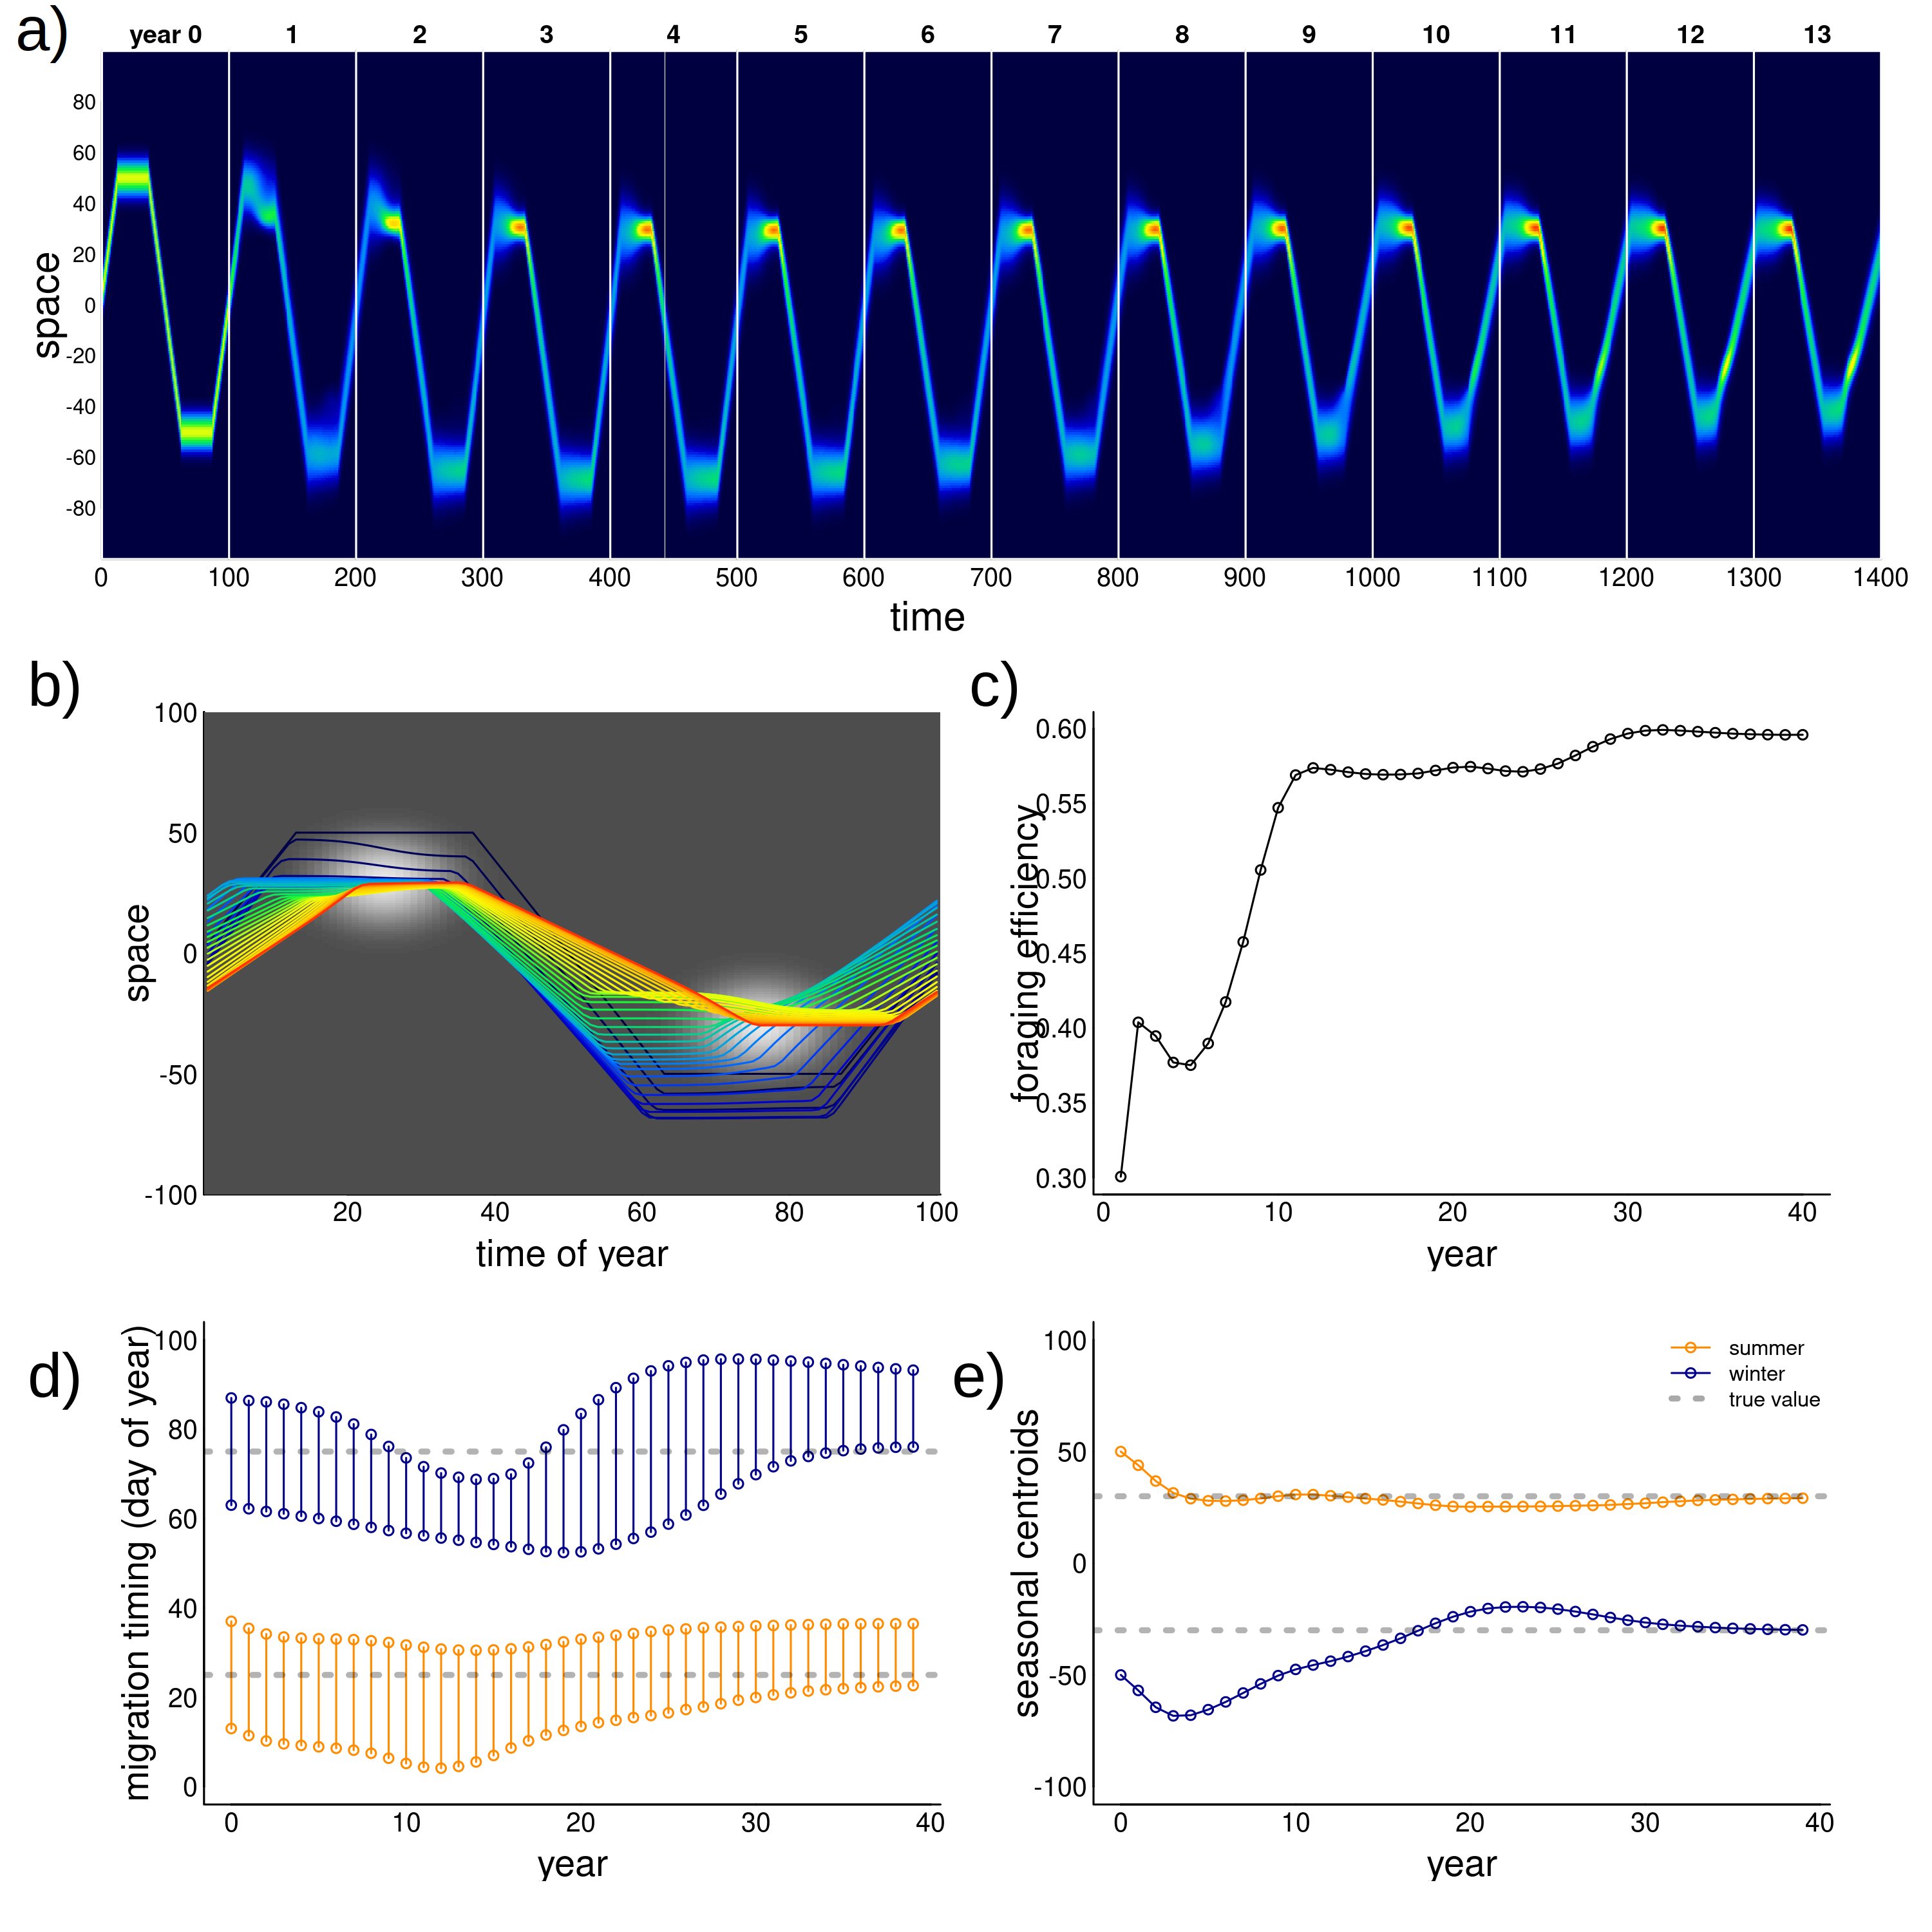
\includegraphics[width = 0.9\textwidth]{figures/example1_adaptation_lettered.png}
		
		\caption{\label{fig_adaptation} Example of adaptation to a shift in resource peak. The initial (year 0) behavior migrates to locations 50 and -50 at days 15 and 60, whereas the resource peak is at 30 and -30, peaking at times 25 and 75. The panels show (a) the first 14 years of the simulation; (b) the centroid of the annual movement of the population is shown in panel b, with dark blue to red colors indicating year 0 to year 40; (c) annual foraging efficiency across years; (d) migration timing parameters for each year, with orange segments indicating arrival and departure from the summering (northern) grounds, and the blue segments indicating timing of arrival and departure at the wintering grounds; (e) migration arrival and departure location across years, with blue and orange indicating winter (southern) and summer (northern) locations.}
	\end{figure}
	
\subsection{Adaptation to resource phenology}\label{results_adaptation}
	
	The ability of this system to attain a stable, migratory state that matches the dynamics of the resource is illustrated in figure \ref{fig_adaptation}. In the illustrated scenario, it takes nearly 40 years to attain an equilibrium, and the eventual steady state is one where the centroid of the migration lines up exactly with the centroid of the resource, and the arrival timing coincides with the \emph{peak} of resource availability. Notably, the path to this equilibrium is somewhat indirect, with the later winter range taking more time to stabilize than the earlier summer range. The eventual steady state is one where the foraging efficiency is relatively high, near 0.6 compared to an initial value of 0.3.  However, the increase in the foraging efficiency was not entirely monotonic, as the system moved through some slightly sub-optimal stages in adjusting its migration behavior. 
	
	We ran this process for 8100 parameter combinations crossing different values of the movement process ($\alpha$, $\beta$ and $\lambda$) and resource characteristics ($\sigma_x$ and $\sigma_t$), and present the total mismatch (TM) against all those combinations in figure \ref{fig_phenologymatching}. In all of these simulations, memory was entirely recent ($\kappa = 0$), since there can be no benefit to relying on a sub-optimal reference memory. We compared a set of diffusion rates $\varepsilon$ between 1 and 8, but only illustrate results for $\varepsilon = 4$. 
	
	A well-matched migration phenology (TM < 5) occurred under very many combinations of parameter values, but all parameters play interacting roles.  Among the more intuitive results are that greater values of $\alpha$ (resource following) lead to an improved ability to match the migration. Resource peaks with larger spatial extent (higher $\sigma_x$) are generally better for migration matching. 
	
	Less intuitive was the high importance of the sociality parameters, in particular the spatial scale of the swarming. Higher levels of social attraction ($\beta$) led to improved migration matching except in those cases where the sociality scale $\lambda$ was high. Thus, for example, at $\lambda = 20$, no simulations at $\beta \geq 200$ managed to acquire or maintain a matched migration. However, at $\lambda = 50$ or $100$, the migration was slightly better matched at high values of $\beta$ (figure \ref{fig_phenologymatching}). The spatial extent of the swarm was a remarkably significant variable. Smaller swarms were able to match migration only at low values of social attraction ($\beta = 200$), and relatively high values of resource attraction ($\alpha \geq 600$).
	
	Random forest analyses, whether on the log of total mismatch or on the classification of a perfect match, uniformly show that the most important variables \citep{Breiman2001} were $\alpha$ and $\lambda$ (4.14 and 4.02 proportional increase in MSE), and the least important was $\sigma_t$, with a 0.5 proportional increase.
	
	Overall, foraging efficiency was strongly correlated with migration matching, as expected. At high mismatch ($>50$), foraging efficiency was low (mean 0.29, s.d.~0.16) compared to the near-perfect matching migrations (mean 0.58, s.d.~0.14). However, somewhat higher mismatch (1 to 5) showed an even higher overall foraging efficiency (mean 0.62, s.d.~0.18 - see also figure \ref{fig_boxplotFE}).
	
	\begin{figure}
		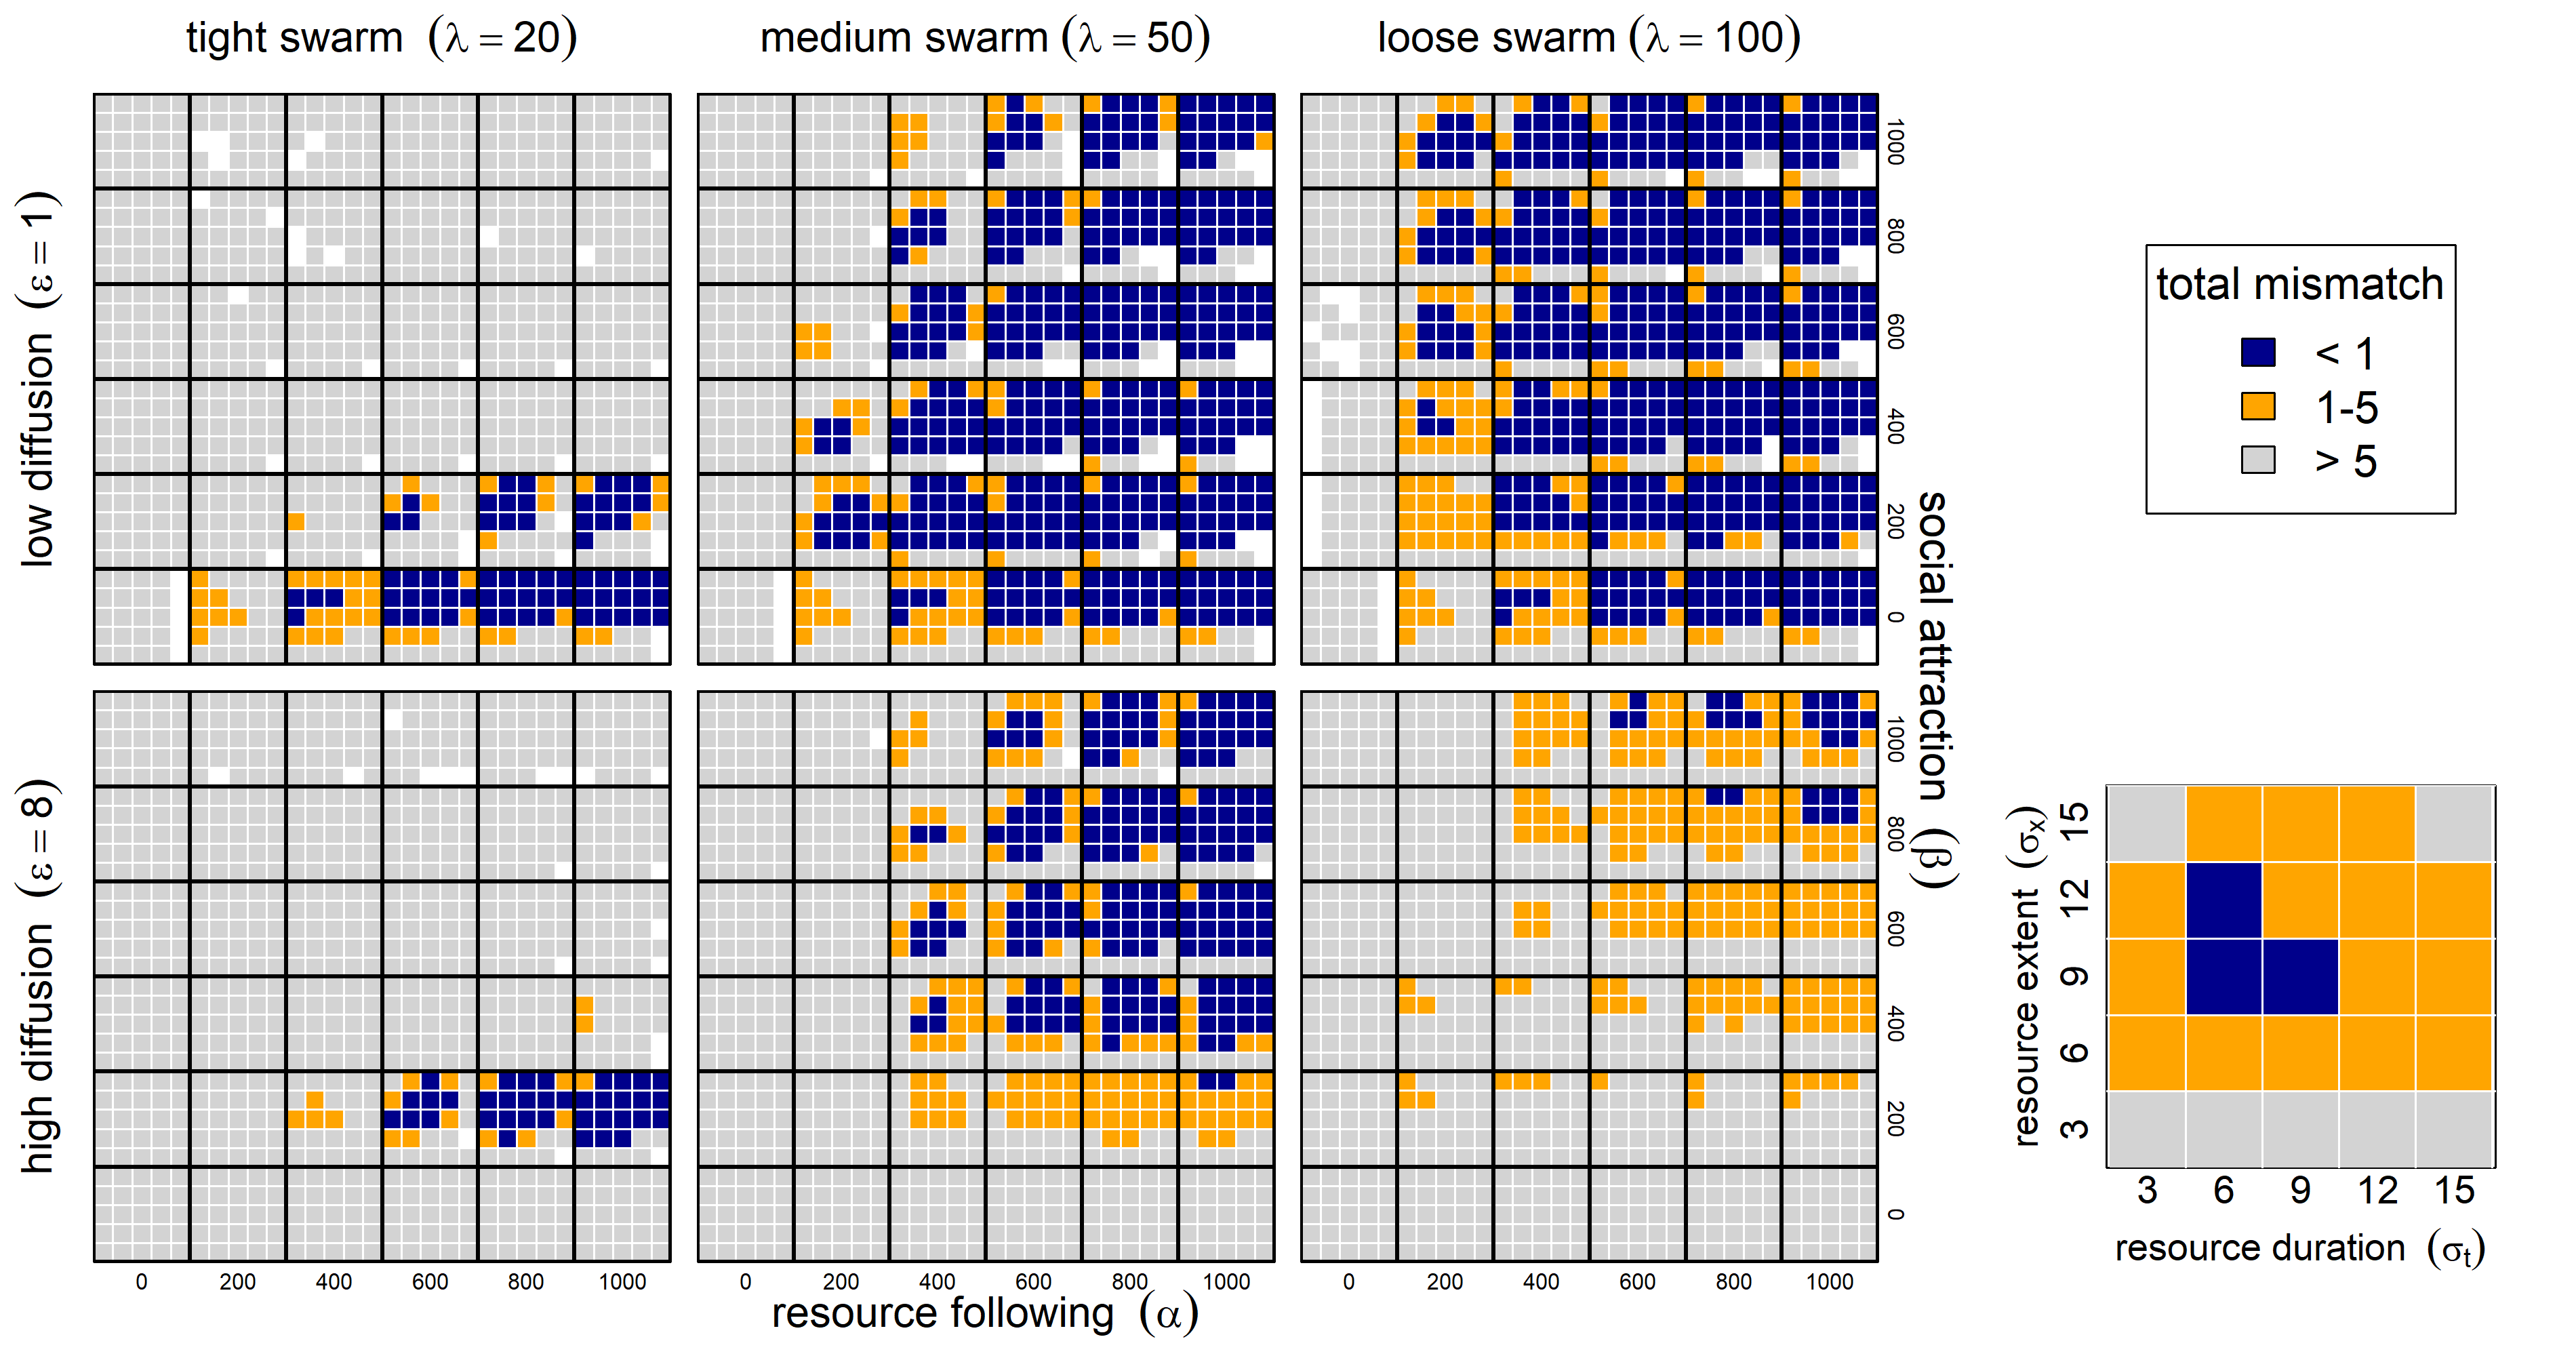
\includegraphics[width = \textwidth]{figures/StabilityResults.png} 
		\caption{\label{fig_phenologymatching} Migration phenology matching across six model parameters. Low and high diffusion ($\varepsilon = 1$ and $8$ in upper and lower panel blocks), tight, medium and loose swarms ($\lambda = 20, 50, 100$) left to right panels. Within each of these blocks, high values of the resource following parmaeters $\alpha$ from 0 to 1000 are left to right, and higher values of the sociality parameter $\beta$ are bottom to top. Within each of the combinations of $\varepsilon, \lambda, \alpha, \beta$, we show results ranging across 5 values of resource duration ($\sigma_t$, 3 to 15 left to right), and 6 values of resource extent ($\sigma_x$, 3 to 15 bottom to top), as in the zoomed-in panel (bottom right; drawn from $\alpha = 200$, $\beta = 200$, $\lambda = 100$). The color scheme reflects the total mismatch, i.e.~the sum of the absolute differences between the migration timing and locations from the resource peak. The white squares represents parameter combinations where the PDE could not be solved for artifactual numerical reasons, that all correspond to a failed adaptation (high mismatch). }
	\end{figure}
	
	\begin{figure}
		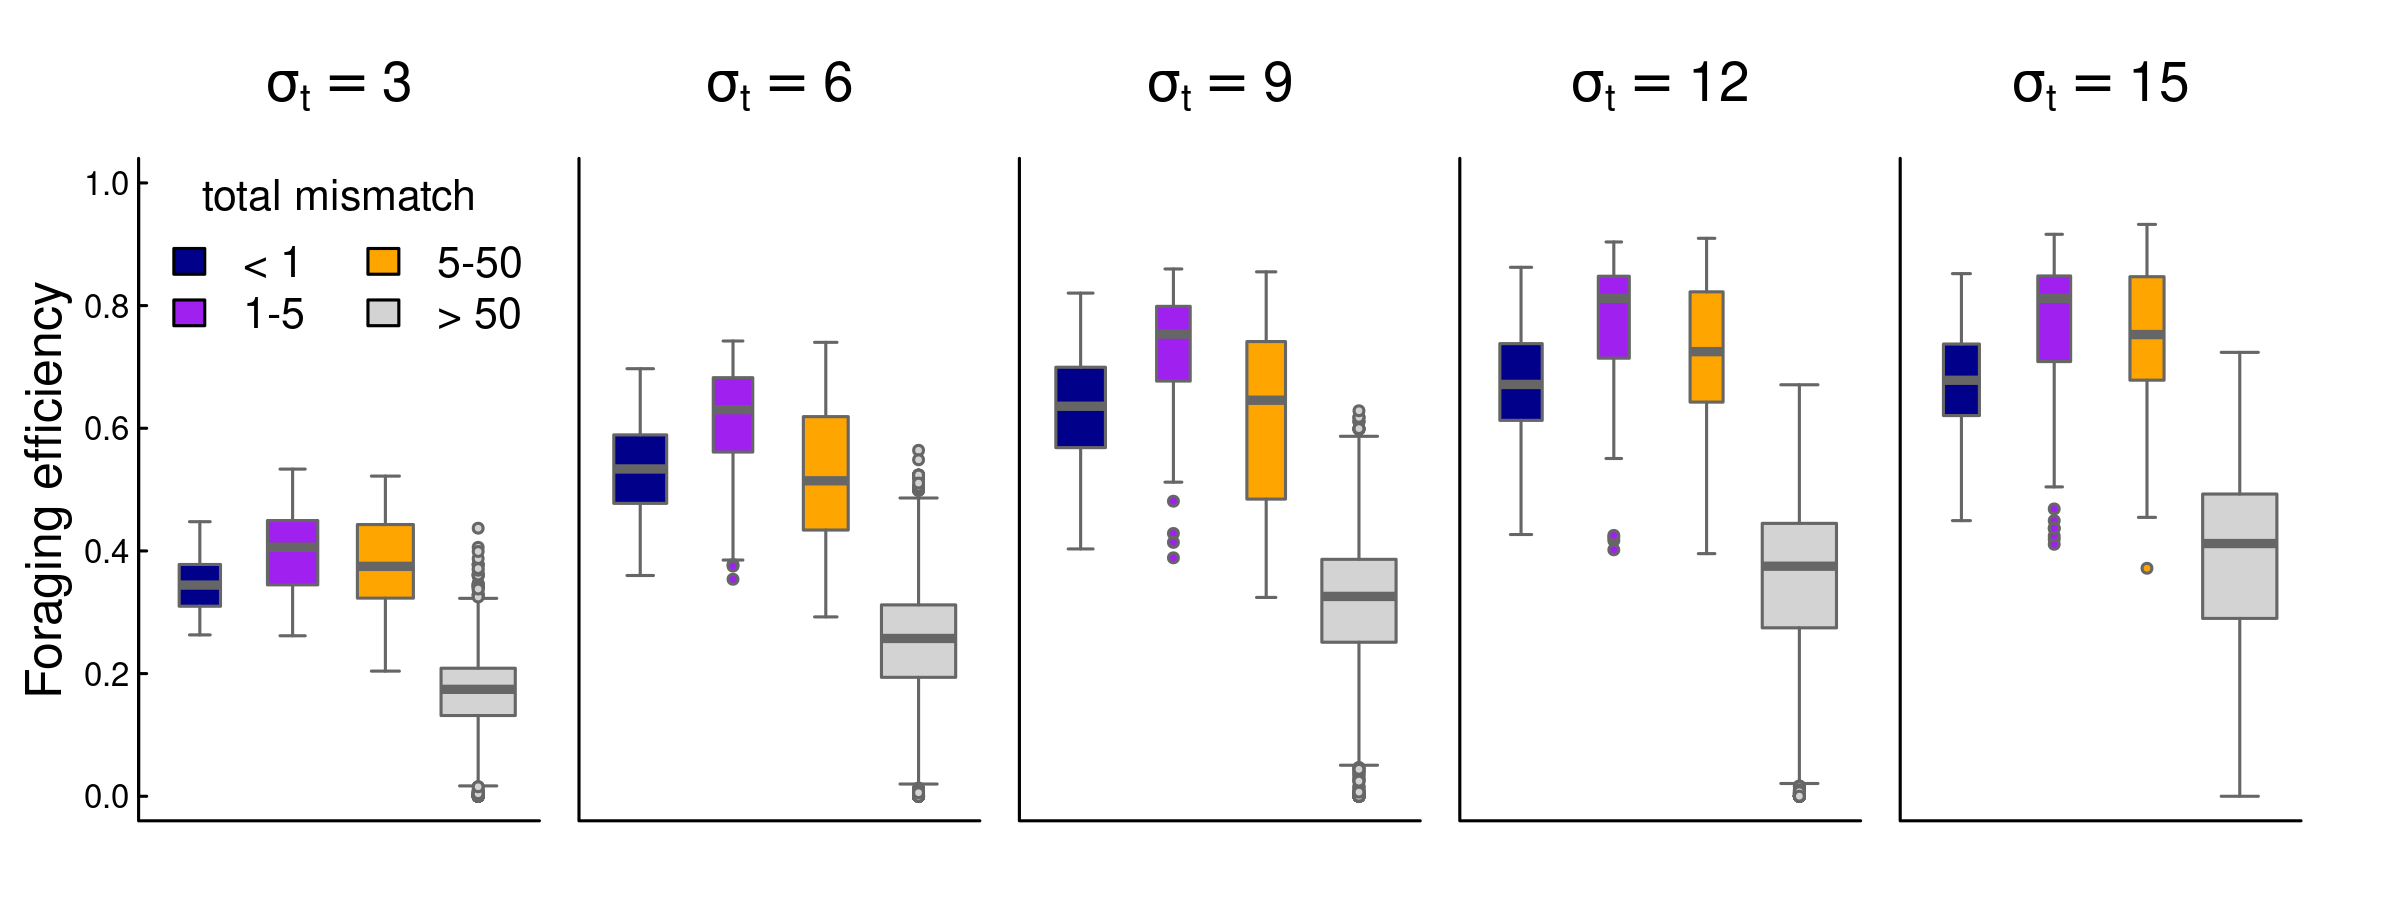
\includegraphics[width = \textwidth]{figures/ForagingEfficiency.png}
		\caption{\label{fig_boxplotFE} Box-plots of foraging efficiency against mismatch across several values of foraging patch duration.}
	\end{figure}
	
\subsection{Learning to migrate}
	
	\begin{figure}
		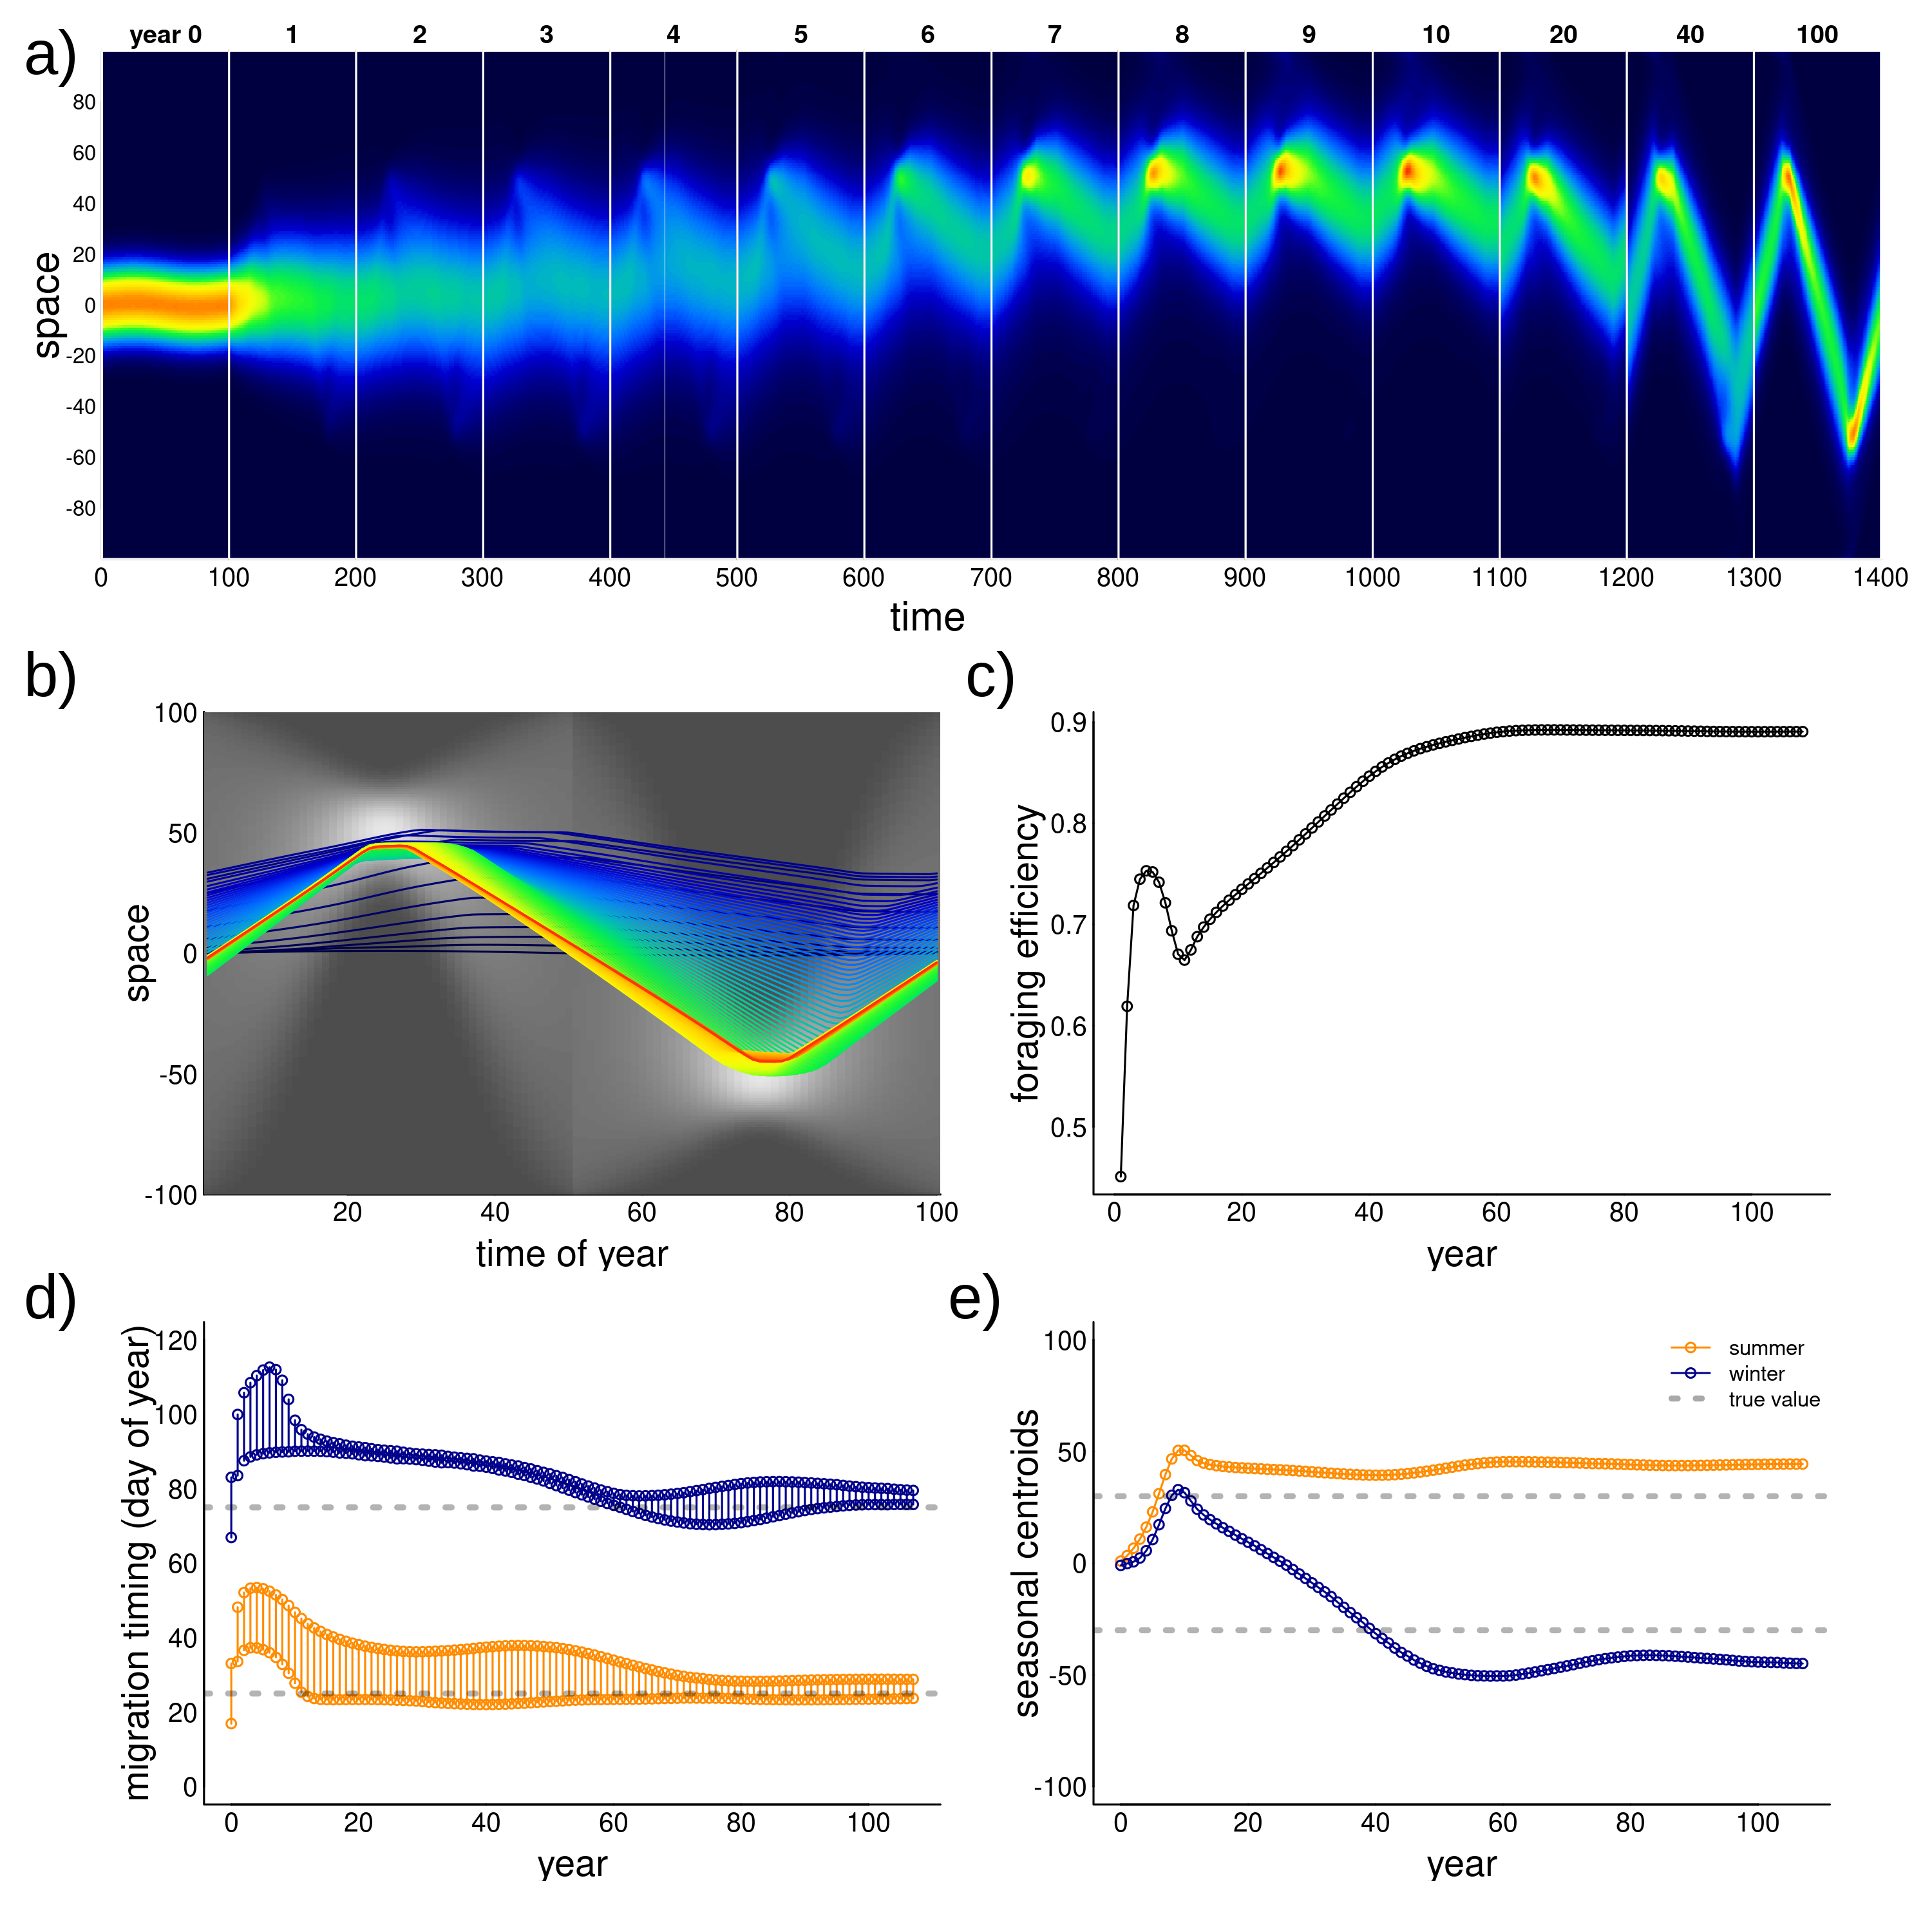
\includegraphics[width = 0.9\textwidth]{figures/example2_learningtomigrate_lettered.png} 
		
		\caption{\label{fig_learningtomigrate} Example of model learning to migrate. The resource is a ``weakly drifting'' resource and the initial (year 0) condition is non-migratory. The simulation was run for 100 years, and a sampling of those years (labeled) are presented in panel a: all years from 0 to 10, followed by 20, 40 and 100. Otherwise, panels are as in figure \ref{fig_adaptation}. Additional parameter values were $\varepsilon = 5$, $\alpha = 500$, $\beta = 50$ and $\lambda = 40$.}
	\end{figure}
	
	Figure \ref{fig_learningtomigrate} illustrates the ability of the model animals to learn to migrate in a weakly drifting resource environment with a narrow pulse of resource peaking at 30 and -30 (at days 25 and 75), but a uniform distribution of resource at times 0 and 50. In order to learn to migrate, the system needed to have a higher exploratory impulse (higher diffusion constant $\varepsilon$), a stronger resource advection (higher $\alpha$) and somewhat weaker sociality (lower $\beta$). The qualitative behavior of this process was to start drifting towards the summer resource, while slowly developing a weak pulse towards the winter resource as well. After first locking in on the summer resource, the winter migration, driven both by high diffusion and high resource following, slowly extended itself until both narrow peaks of resource were consistently reached.
	
	The model had, in general, a difficult time learning migration from a non-migratory initial condition. Out of 4047 successful runs, only 4 attained mismatch below 1, and 130 below 5. Conditions that were more conducive to learning migration were pulses of \emph{longer} duration (high $\sigma_t$), but \emph{smaller} in scope (low $\sigma_x$), suggesting that the feedback that encourages migration needs to be compact in space but long enough in duration to lock in to the memory.
	
\subsection{Directional climate change}
	
	\begin{figure}
		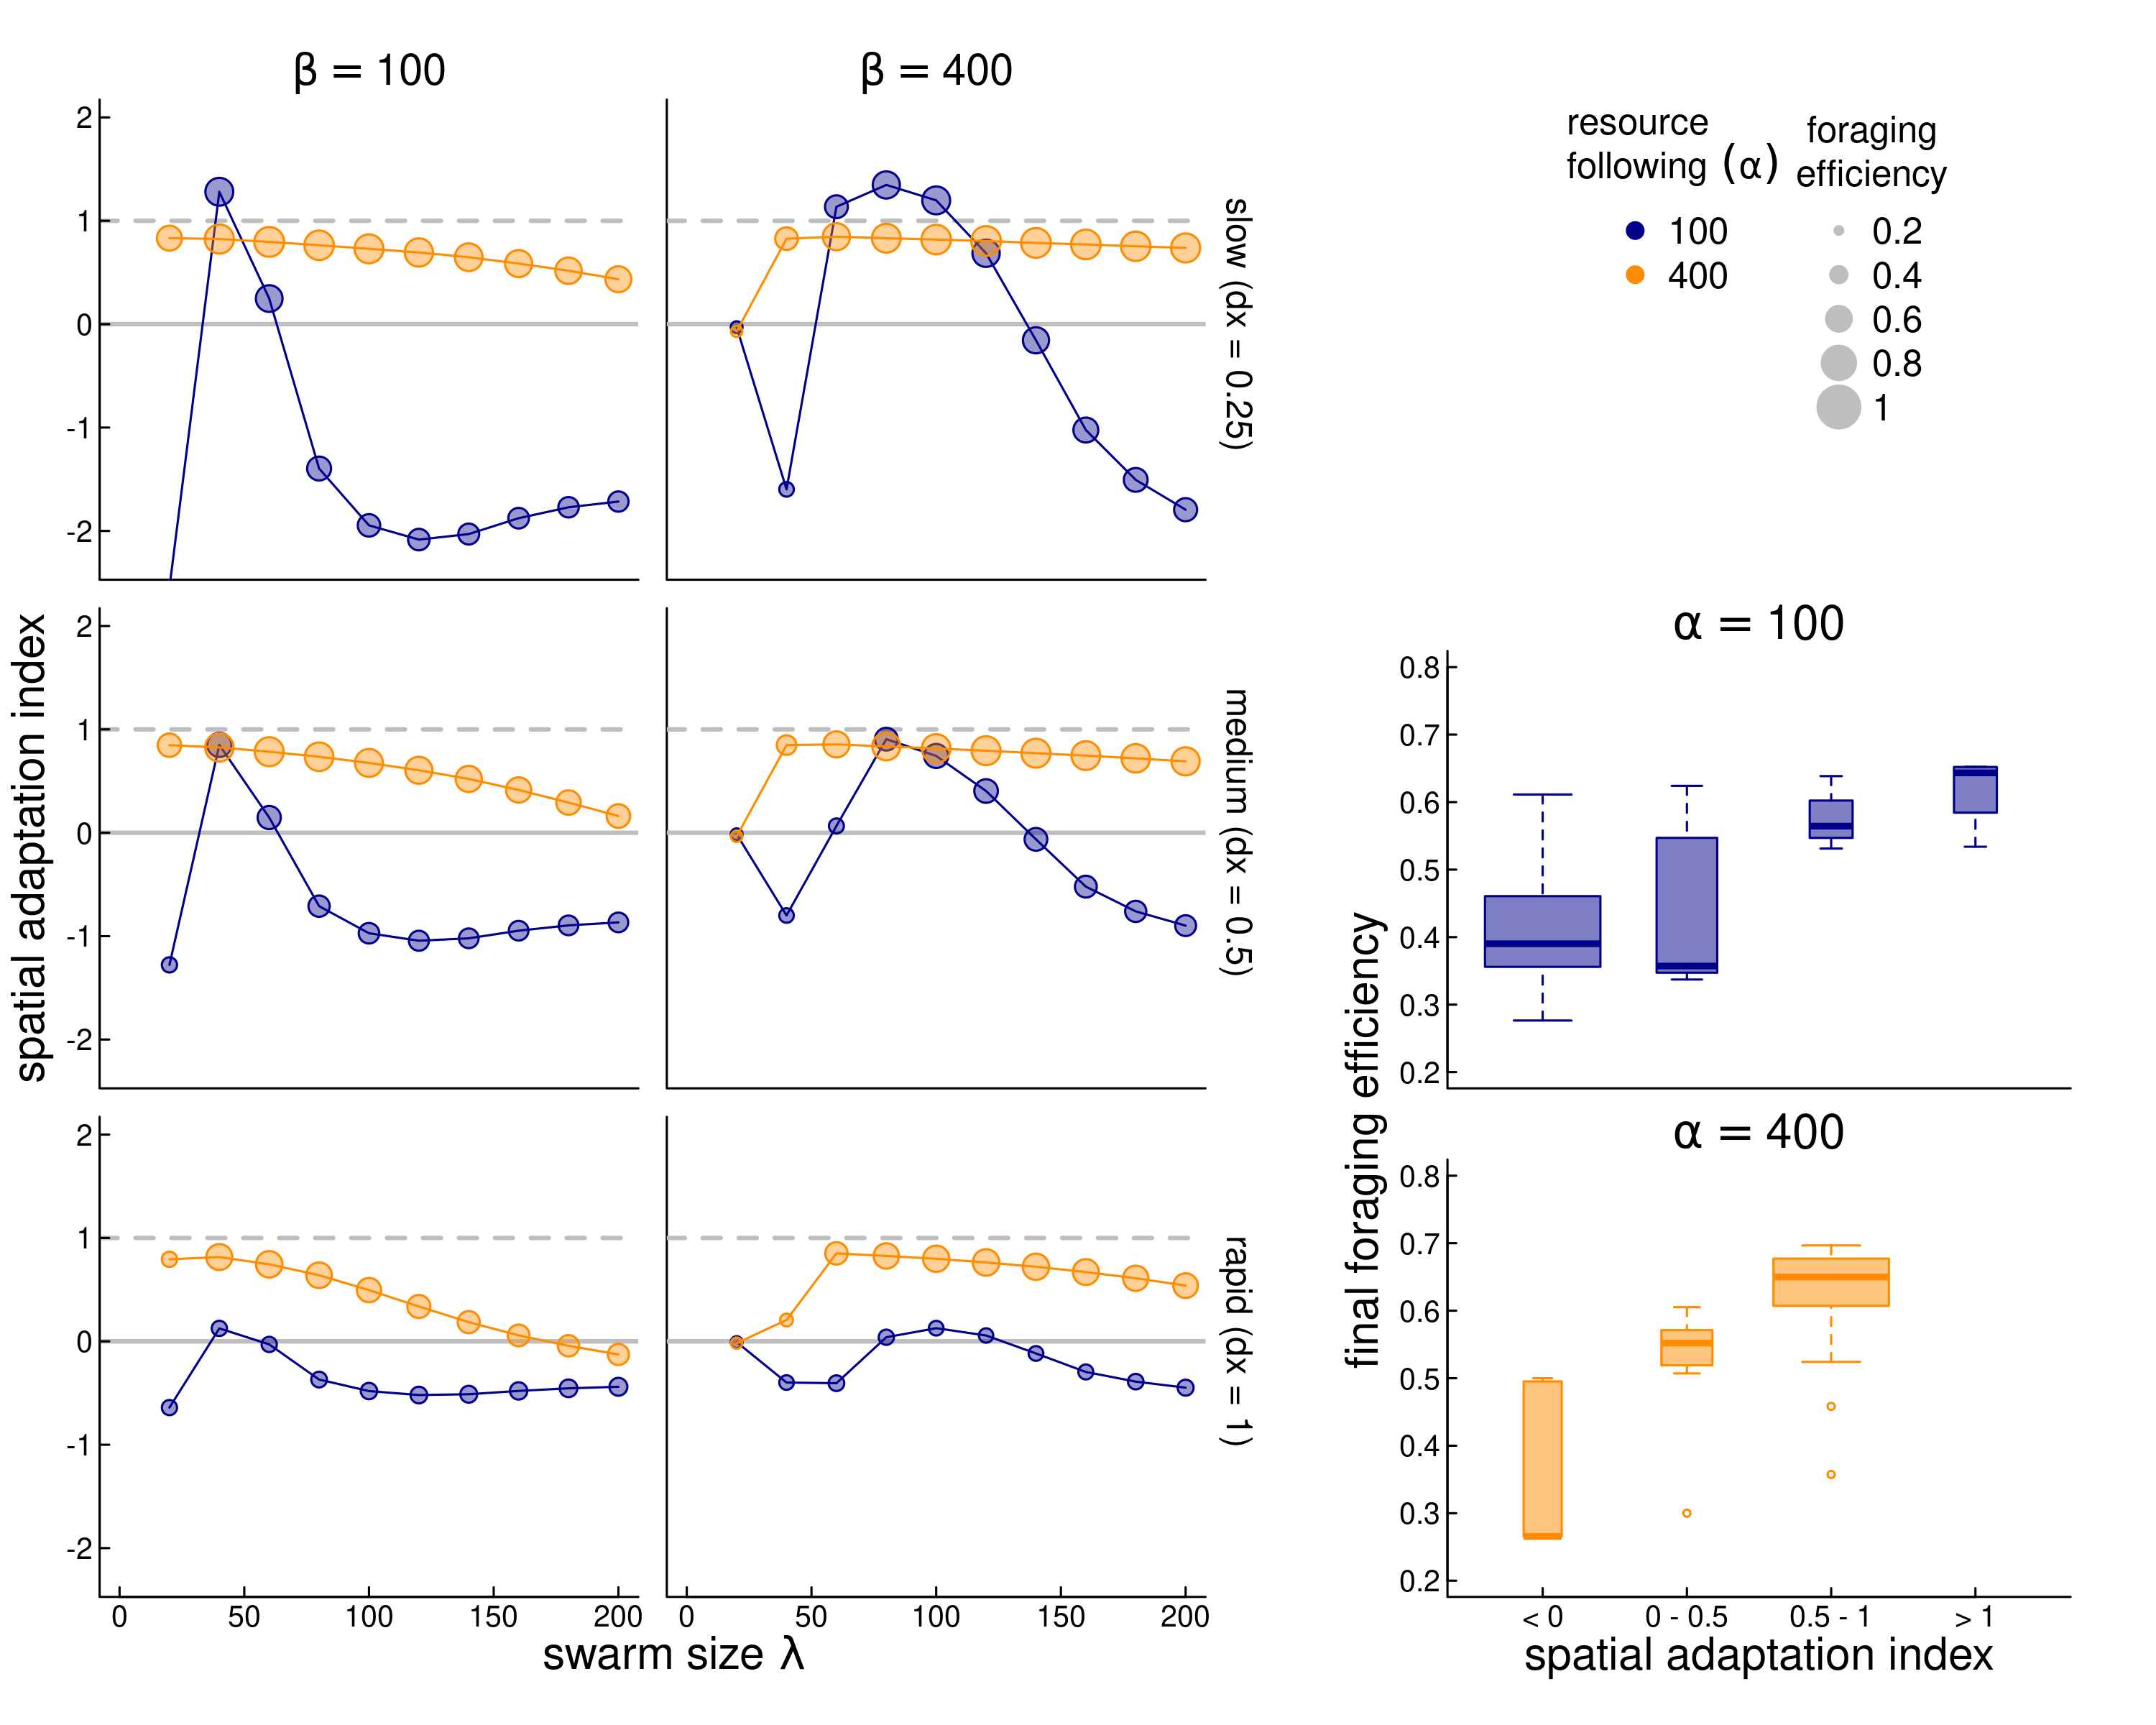
\includegraphics[width = \textwidth]{figures/SpatialClimateChange.png}
		
		\caption{\label{fig_adaptationclimate} Adaptation to a steadily drifting resource. In three scenarios, the spatial coordinates of the resource drift by 0.25, 0.5, and 1 unit per year (top to bottom, respectively). The y-axis is the spatial adaptation index (SA), i.e.~the trend of the memory-driven migration divided by the resource drift trend. Values near 1 indicate a behavior that keeps up with climate change, values near 0 indicate no change in migration behavior, and negative values indicate a trend that is opposite to the climate trend. We compare across spatial scales of sociality ($\lambda$ - x-axis), for low and high values resource following ($\alpha = 400$ and $100$ - orange and blue dots) and low and high values of sociality ($\beta = 100$ and 400, left and right panels). The size of the circles is proportional to the foraging efficiency of the resulting parameter combinations. The bottom-right boxplots indicate the final year foraging efficiency against SA; purple and blue boxes indicate the highest values, orange and gray lower values.}
	\end{figure}
	
	To assess the ability of the system to adapt to a trending climate, we generated scenarios with slow, moderate and fast outward directional shifts in the resource peak (0.25, 0.5 and 1 units / year, respectively). We then assessed 40 parameter combinations for each of those scenarios, high and low values of resource following ($\alpha = 400$ and $100$), high and low values of sociality ($\beta = 400$ and $100$) and 10 values of the spatial scale of sociality ($\lambda = 20$ to $200$). The spatial and temporal scale of the resource pulses were fixed to $\sigma_x = 12$ and $\sigma_t = 6$, a combination which analyses in section \ref{results_adaptation} showed were generally ``easy'' to adapt to. We computed the adaptation index and foraging efficiency for each of the 120 runs (figure \ref{fig_adaptationclimate}). We were interested in the dynamics against $\lambda$ due to the consistently high importance of this parameter for matching migration in steady states. Our main index of interest was the spatial adaptation (SA) to trends. 
	
	As figure \ref{fig_adaptationclimate} shows, higher values of resource following ($\alpha = 400$; orange circles) are nearly universally better for keeping up with climate change (SA values near 1). Furthermore, when combined with high sociality ($\beta = 400$; right panels), nearly all parameter combinations do a good job keeping up with climate change (SA values ranging between 0.53 and 0.85 for a swarm size greater than 50). However, that maximum value is still less than 1, suggesting that truly matching a steadily drifting trend is very difficult. Smaller social spatial scales ($\lambda < 50$) have a very hard time adapting when the social attraction is high, but do fairly well when social attraction is low. Larger sized swarms do progressively worse across more parameterizations, e.g.~in the most rapid climate change scenario, the SA drops from 0.83 to -0.13 as the swarm increases in size from 40 to 200 (encompassing, essentially, the entire spatial domain).
	
	A rather more dramatic pattern is visible for the lower foraging attraction scenario ($\alpha = 100$; blue circles). Notably, no parameter combination at this value comes close to keeping up with the rapid climate change (SA range -0.64 to 0.13). For slower climate change, however, there is a window of values for the swarm size between 40 and 80, where the SA \emph{exceeds} 1, but then crashes quite rapidly to negative values of SA as that swarm size increases. These ``super-adaptive'' processes indicate a unique sweet spot where a swarm is large enough to capture and adapt to the drifting resource, but not so large that the information gathered in a given year is too weak to adjust the migratory behavior in a following year.
	
	As anticipated, better adaptation to the drifting resource correlated strongly with higher foraging efficiency (inset boxplots).\\
	
\subsection{Reference memory and stochasticity}
	
	While recent memory can be helpful for adapting to a single novelty or a smoothly changing conditions, we hypothesized that more conservative approach that relies on a reference memory may be beneficial when conditions change stochastically. We tested this hypothesis by solving a set of models across a range of $\kappa$ values fom 0 (all recent memory) to 1 (all reference memory). In these scenarios, we ran the system for as many years as needed with no stochasticity to acquire a stationary state (i.e.~similarity index greater than 1-1e-6). We then used the stationary state as the reference memory, and then ran the process for an additional 50 years with a stochasticity (i.e.~standard deviation in peak location of the resource) ranging from 0 to 12, and present the resulting average foraging efficiency (figure \ref{fig_stochasticity}).
	
	Overall, as expected, the greater the stochasticity, the lower the foraging efficiency.  Further, as we predicted, highest level of $\kappa$ can significantly help foraging efficiency, with some variation across the spatial scale of sociality, especially in more highly stochastic scenarios. When that scale of sociality is high enough ($\lambda = 120$, blue colors) there is greater probability of overlap with a stochastic resource, and a conservative, stable migratory regime is much more beneficial in the long run. \\
	
	\begin{figure}
		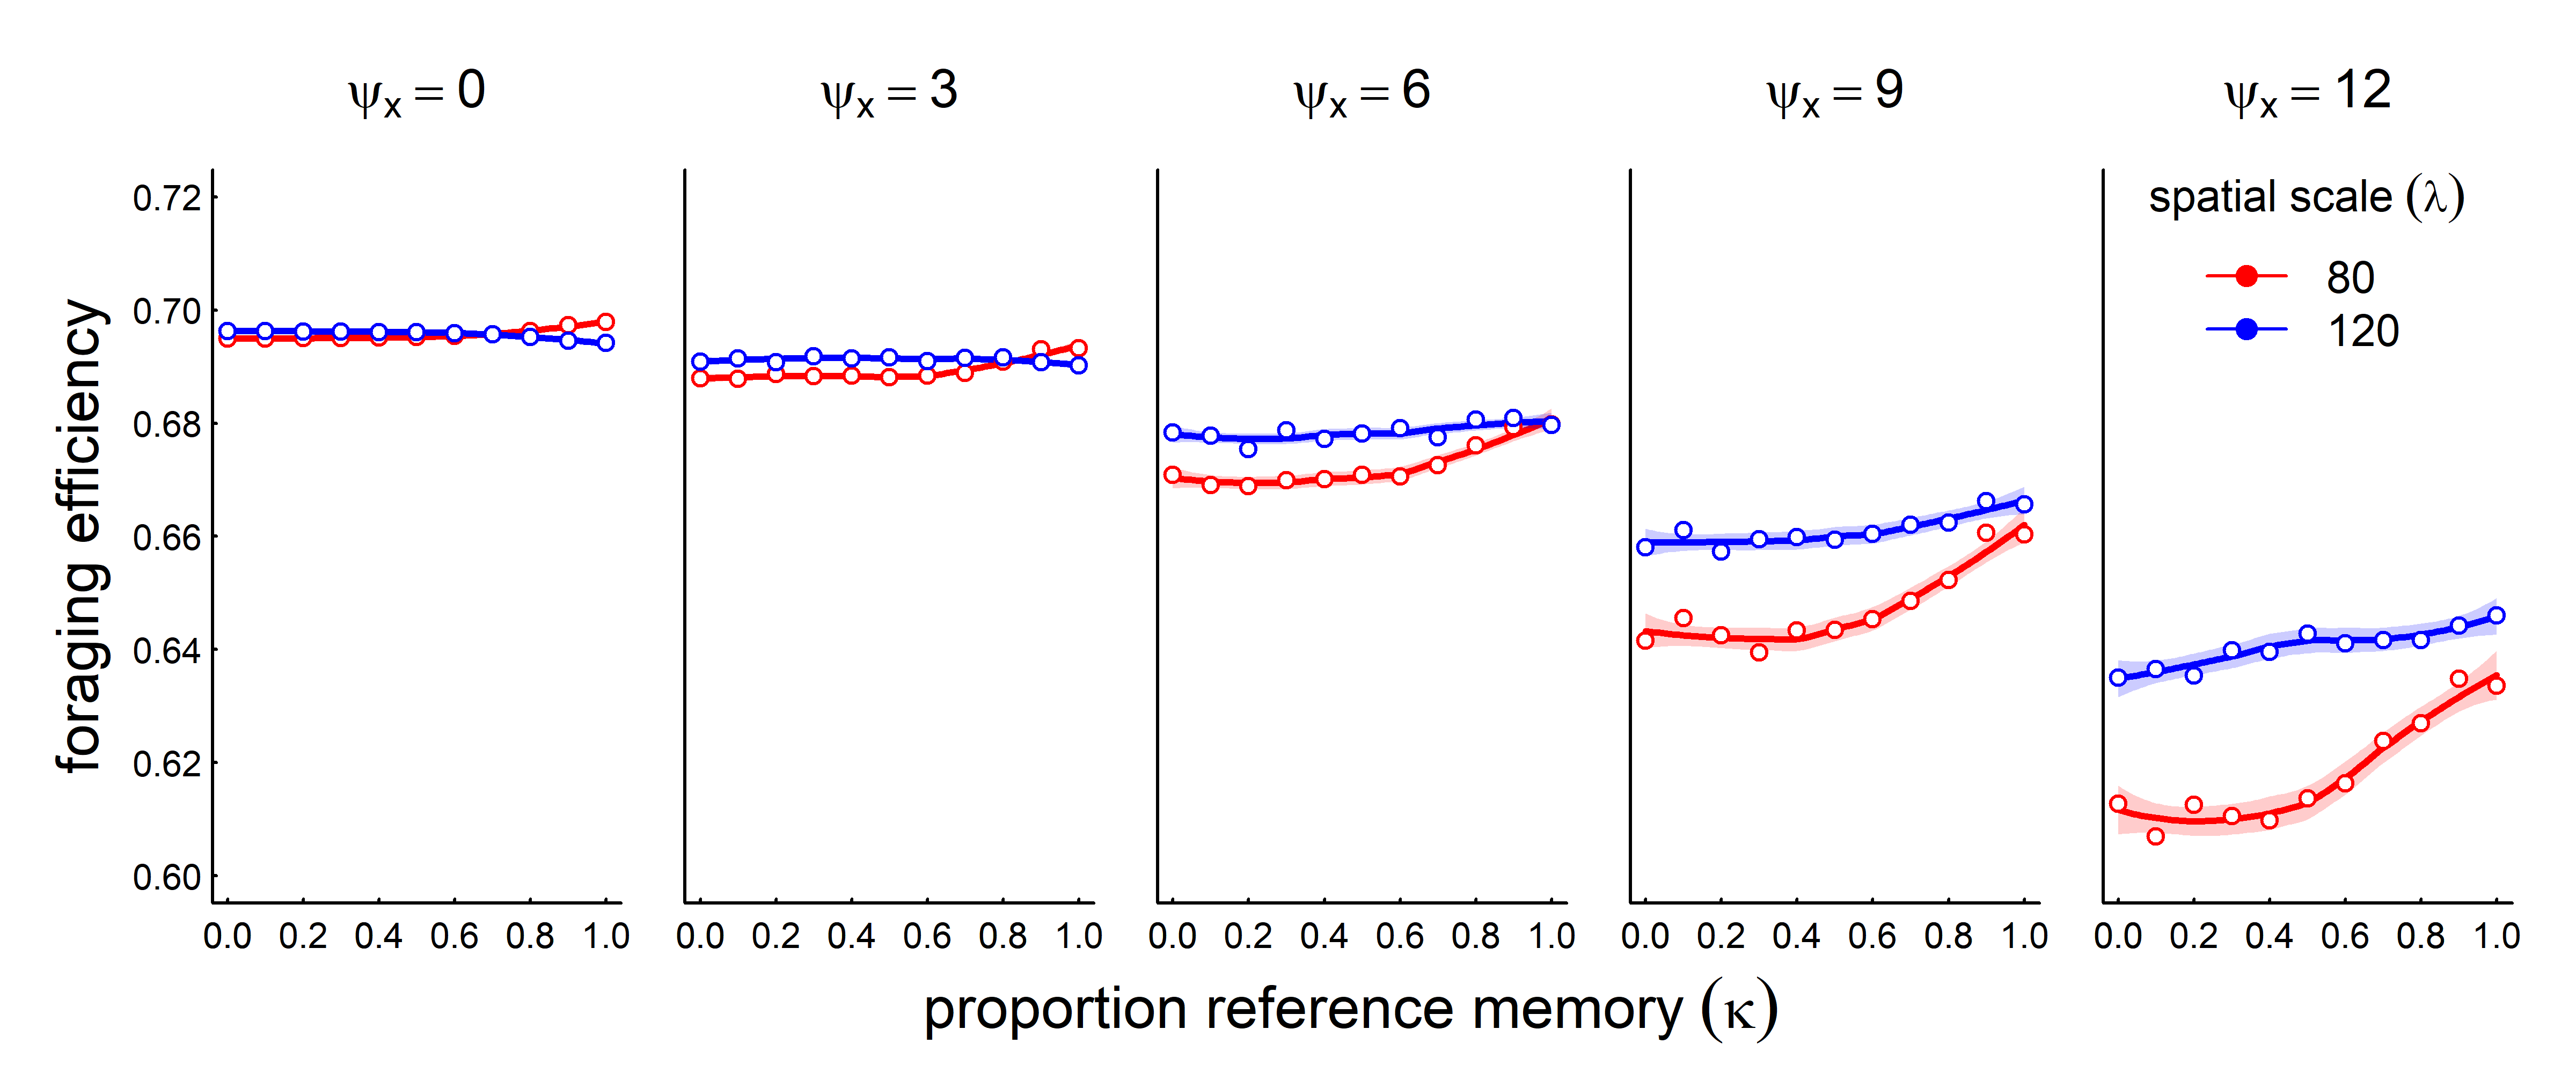
\includegraphics[width=\textwidth]{figures/stochasticity.png}
		
		\caption{\label{fig_stochasticity} Foraging efficiency (FE) across various values of reference memory $\kappa$ (x-axis) for increasing amounts of interannual stochasticity ($\psi_x$, panels left to right), and two values of sociality spatial scale $\lambda = 80$ and $120$. For the processes with non-zero stochasticity ($\psi_x > 0$), the process was run 90 times for values of $\kappa$. Points represent the average of the FE's across all 50 years and 90 replicates. In these scenarios, the resource following parameter $\alpha = 100$, the social attraction $\beta = 400$ and diffusion $\varepsilon = 4$. Note that the y-axis scale is constrained over a relatively narrow range (0.6-0.7). } 
		
	\end{figure}
	

\subsection{Stochasticity and trends}
	
	We added 30 years of directional trends to the variously stochastic process described above, and assessed the adaptation index against the reference memory parameter $\kappa$ (figure \ref{fig_trendstochasticity}). Over-reliance on reference memory ($\kappa = 1$) by definition does not allow the system to keep up with climate change, leading to an adaptation index of 0. However, in many cases a balancing of recent and reference memory ($\kappa$ value between 0.6 and 0.8) in many cases was slightly but significantly better than relying entirely on recent memory. The smaller spatial scale (in the selected parameter space) does a generally better job than the larger spatial scale at lower stochasticity. At higher level of stochasticity, however, the larger spatial scale outperforms the smaller spatial scale, which completely loses track of the climate change.
	
	\begin{figure}
		
		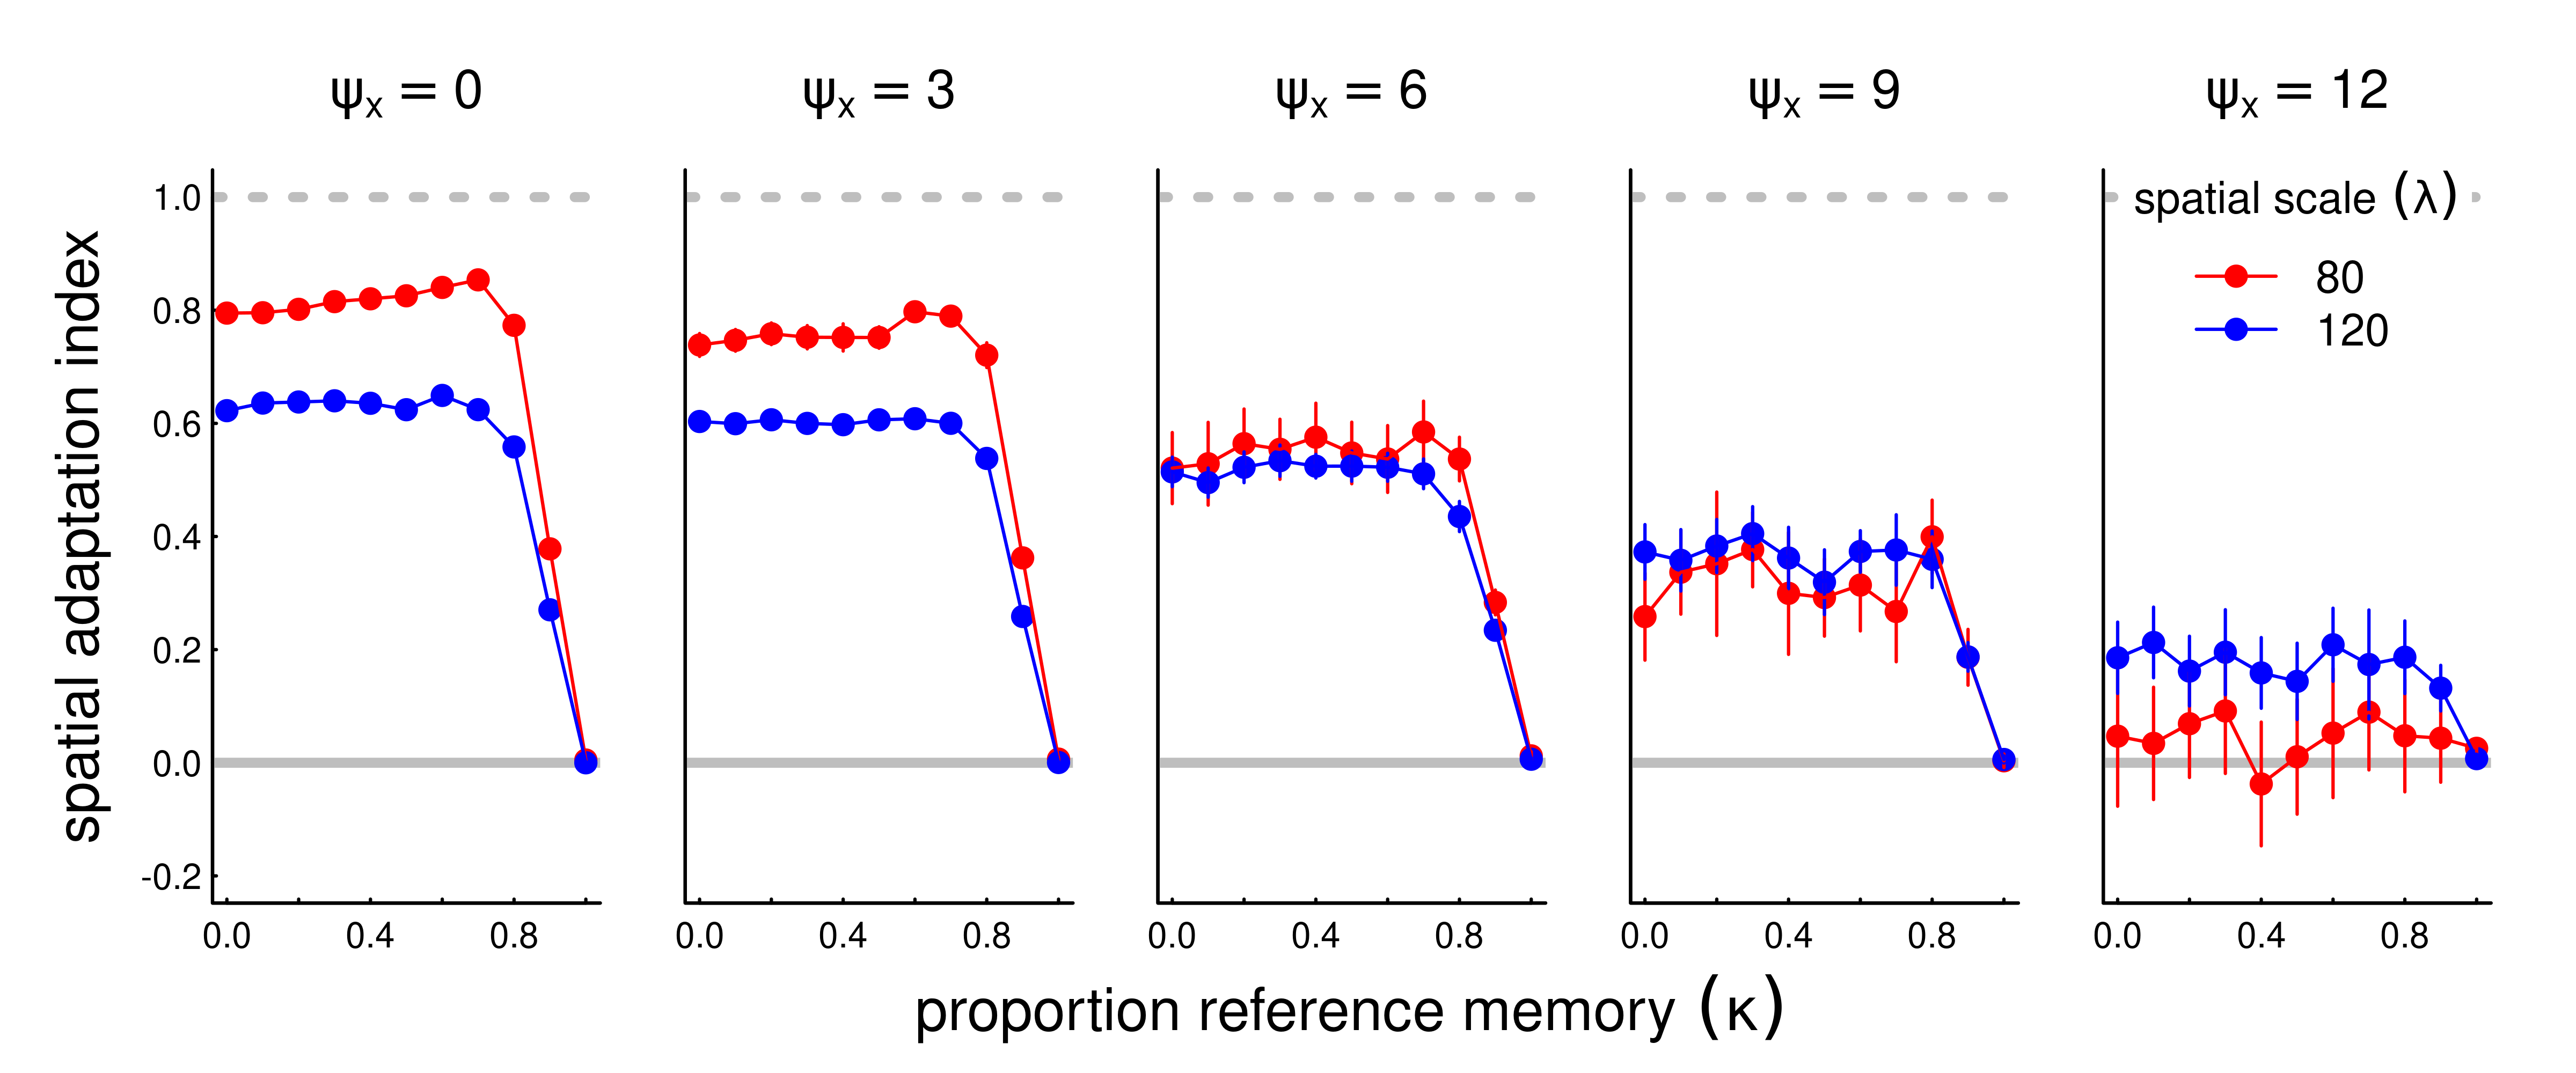
\includegraphics[width=\textwidth]{figures/TrendStochasticity.png}
		
		\caption{ \label{fig_trendstochasticity} Role of reference memory in adapting to climate change for increasingly stochastic resource dynamics. We ran the model with a moderate rate of climate change (mean shift: 0.5/year) at five increasing levels of stochasticity (inter-annual standard deviation of resource peak 0, 3, 6 and 12, left to right panels). For non-zero stochasticity, we ran the process 30 times and present the mean and standard error of the spatial adaptation index across various values of the reference memory parameter $\kappa$: where $\kappa = 0$, the system modifies its migration based entirely on recent experiences; at $\kappa = 1$, the memory never changes from the reference memory. Other parameter values are resource following $\alpha = 100$, social attraction $\beta = 400$, and diffusion $\varepsilon = 4$.}
		
	\end{figure}
	
\section{Discussion}
	
	Animals navigate complex, dynamic and patchy environments. When there is a strongly localized and seasonal component to the resource dynamics, movement strategies limited to straightforward resource-following taxis necessarily fail to efficiently exploit available resources. It is in these cases, quite common in the natural world, that seasonal migration becomes a viable, even necessary, strategy.  However, when resources start shifting in space and time -- as is occurring at an accelerated pace with recent global climate change -- the migration phenology itself must exhibit some plasticity. It is our conjecture that this plasticity is facilitated by a memory-driven process in which recent experiences inform strategic behaviors in subsequent years. 
	
	By allowing a population to adjust its migratory behavior based on recent experiences with the resource location, the model we presented here emulated (a) the successful navigation of an environment with temporally and spatially isolated seasonal resource patches, (b) the emergence of a migratory behavior from an essentially resident or naive initial condition, and (c) some intrinsic robustness to changes in those environmental resources, whether steadily shifting trends or inter-annual stochasticity. The relatively simple, social and memory-driven mechanism was able to adapt to long-term changes in resource dynamics, even with inter-annual stochasticity, and may thereby provide a framework with which the interaction of memory, movement, social and resource dynamics can be further explored.  % In a generalized way, it captured all three fundamental types of migration plasticity: the \textit{where}, the \textit{when} and the \textit{whether} \citep{Xu2021}. 

	Importantly, our model was in no ways evolutionary, as it contained no birth-death processes or selection pressures. Thus, we used foraging efficiency as a convenient metric of the utility of migration, though this was not a measure explicitly maximized by the model. Other metrics, such as foraging efficiency in a given season, or probability of survival or reproduction relative to resource availability \citep{Bauer2020} may respond differently across model parameters and could be useful in understanding the relative success of alternative migratory strategies in different contexts. However, the overall annually averaged foraging efficiency metric provided the broadest linkage between resource dynamics and animals' locations and was consistent with the minimal biological assumptions and generality of our framework. \\


\subsection{Adaptation and resiliency}
	
	Our goal was to understand the combinations of factors that lead to a resilient migration behavior. The model we describe was a final iteration of a sequence of models which failed to develop or maintain social migration behavior. For example, in earlier versions memory was modeled as an attractive advection mathematically identical to the resource attraction, but with the attractor being the location of the population in previous years.  These models proved to be inefficient at generating a consistent social migratory behavior, i.e. only under very specific parameter combinations and ``easy'' conditions was a migratory equilibrium, and that equilibrium was highly unstable to perturbations.  Only a clear, directed advective process with an explicit seasonal signal (i.e.~the remembered migration timing, rates, and targets which were remembered in our model) could generate the patterns we aimed to capture.  This suggests, somewhat indirectly, that migration behavior is unique as a fundamental, long-term, and risky strategy, profoundly different from the kind of tactical resource response which governs shorter-scaled animal redistributions. 
	
	Similarly, iterations of the model that did not have some amount of social cohesion tended to diffuse away without establishing a consistent, migratory stationary state. In fact, sociality parameters -- in particular, the spatial scale $\lambda$ -- were, unexpectedly among the most important parameters for determining the resiliency of the process. Populations with small spatial scales tended to have a more difficult time locking in to an adaptive migratory pattern, and only when social attraction was relatively weak. On the other hand, overly large spatial scales compromised the ability of the process to track climate change, due to a dilution of the population's ability to concentrate over available resource patches and remember the corresponding benefits.  
	
	The ability to adapt a migration also depended strongly on properties of the resource dynamics. In particular, the reinforcement of memory and foraging is strongest when patches are concentrated in time, but relatively large in space. Interestingly, in most stable patterns, the eventual targeted migration arrival time coincided with the \emph{peak}, rather than the beginning, of the resource dynamic. This indicates that the long-distance social migration behavior may be particularly reinforced when the targeted resource is very sudden. This is the case for the rapid green-up that occurs in high latitudes as snow recedes in tandem with extended day lengths leading to an intense green-up period \citep{Park2020} or, for example, when resources are linked to the short-duration early blooming phenology of very particular plants \citep{Post2007, Renner2018}. 
	
	Even with no strong intrinsic propensity to migrate and a weak phenological resource pulse to follow, our model captured the ability to acquire a strong and adaptive migration behavior (figure \ref{fig_learningtomigrate}).  Learning migration, howewer, requires a very strong resource attraction, higher levels of exploratory behavior (e.g.~diffusion, and larger spatial scale of sociliaty), and -- often --- many more years, findings that echo empirical observations \citep{Jesmer2018}. 
	
	Despite the ability of the process to adapt under many stable conditions, our migration model (and, perhaps, migration behaviors in general) can also be considered somewhat fragile. Under many shifting conditions, e.g.~increasing stochasticity, rapidly shifting resources, a shift in some of the system parameters, or even a shift in the spatial and temporal extent of resources, migration can collapse and turn into a non-migratory, residential behavior (figure \ref{fig_phenologymatching}). This sensitivity may explain why partially migratory populations are so common and, apparently, evolutionary stable \citep{Berthold1999, Chapman2011}, as well as the wide range of migration plasticity shown in wild populations, even within a species \citep{Xu2021}.\\
	
	
\subsection{Biological interpretation of parameters}
	
	Diffusion-advection models of animal movement and redistribution are grounded in the general idea that animal movements, somewhat like movements of physical particles, combine random (diffusive) components with directed (advective) components \citep{Skellam1951, Turchin1998, Okubo2001}. While direct relationships between diffusion models and movement data are somewhat tenuous \citep{Gurarie2011,Potts2020}, as a theoretical tool for exploring processes they are invaluable for their versatility and the relative ease of numeric computation of the partial differential equations (PDEs) that describe them mathematically. % Refinements to diffusion-advection equations have revealed conditions under which non-local information gathering \citep{Fagan2017} and behavioral switching may confer foraging advantages \citep{Fagan2019}, in particular when resources are dynamic and patchy. While diffusion models that incorporate social movements (swarming, schooling, herds) have been well-studied \citep{Okubo1986, Gruenbaum1994, Mogilner1999}, the interacting role of memory and sociality in a specifically migratory framework has been relatively unexplored. 
	
	Despite its evident abstraction, our goal was to develop a model where all parameters have well-defined biological interpretations. The diffusion ($\varepsilon$) captures short time-scaled randomness of movement, reflecting exploratory and short-term dispersive behavior. The foraging advection strength ($\alpha$) captures the attraction of the population to better quality resources at a relatively large scale. These two parameters, the basic ingredients in diffusion-advection models of animal movement, have direct parallels to empirically estimated properties of animal behavior: diffusion is closely related to families of random walk models \citep{Gurarie2011} while the advective taxis is related to the step and resource selection functions that are routinely estimated from movement data \citep{Potts2020}. The spatial scale of the social group ($\lambda$) captures the spatial extent of the population, i.e.~a population-level home range \citep{Noonan2019}. We note, however, that diffusion-advection models can also be interpreted as a probabilistic description of a single individual's movement. In this case, $\lambda$ would correspond to an individual home-range and $\beta$ would be an individual's tendency to be drawn to the center of that home range, akin to an individual migratory Ornstein-Uhlenbeck process \citep{Gurarie2017}.
	
	The sociality parameter ($\beta$) quantifies the strength of an individual's desire to approach the center of the social group. While this parameter is not typically measured, it may in principle be possible to estimate in a manner analogous to step-selection function by replacing environmental variables with presence of conspecifics as a covariate. The ratio between $\alpha$ and $\beta$ can be interpreted as the relative importance of foraging to social cohesion, which appears to be important in predicting the resilience of migration. 
	
	Migration timing, rate, and seasonal range location parameters can be straightforwardly estimated from movement data \citep{Cagnacci2015, Gurarie2019} and synchrony of migration timing and site fidelity are well-documented for many migratory species \citep{Joly2021}. Thus, for example, \citet{Gurarie2019} explicitly estimated the ranging area, timing, and seasonal range locations for migratory caribou, identifying the kind of inter-annual variation that is reflected in the stochastic scenarios explored here, as well as trends in timing. 
	
	The reference memory parameter $\kappa$ is, of course, impossible to observe directly.  Our model does, however, allow us to explore in an heuristic way the conditions under which a strong cultural tendency to migrate with certain fixed patterns can help a population hedge against stochasticity \citep{Abrahms2019,Fagan2019b}. An extremely conservative behavior is the best way to hedge against stochasticity with no directional changes (high $\kappa$ values in figure \ref{fig_stochasticity}), as there is no benefit to change behavior based on recent experiences if they provide no information about future conditions. However, this extreme conservatism is, by definition, incapable of adapting when there is a consistent shift in resource distribution (figure \ref{fig_trendstochasticity}).  In cases where both processes are occurring, we did see a slight improvement in adaptability when long-term reference memory was balanced against a strong response to recent experience (see peaks in \ref{fig_trendstochasticity}). 
		
	Clearly, our exploration of the model was not exhaustive.  We did not explore, for example, the resilience of the migration process to changes in resource timing, which would correspond to the widely observed earlier onset of spring as measured by green-up and flowering phenology \citep{Cleland2007}. We hope that making the model available, including via the interactive interface, will facilitate further independent exploration of these processes.  \\
	 	
\subsection{Social learning and collective knowledge}	
	
	Models have shown that collective knowledge is important, if not essential, to the evolution and process of migration \citep{Shaw2013, Guttal2010, Berdahl2018}. Many migratory organisms are social, and social learning is an acknowledged, non-genetic method for transmitting information \citep{Kashetsky}. Furthermore, the general role of social learning for improving a population's ability to track resources has been studied not just in animal systems, but in synthetic systems inspired by social behavior of animals such as optimization heuristics algorithms and the study of swarm robotics \citep{Sahin2005, Brambilla2013}.  Because our model is not individual-based, we can not identify any specific mechanism (e.g.~leader-follower) of social information transfer.  But, in a generic way, our model assumes that migration is driven by a collective decision for the timing and locations of seasonal ranges, consistent with the known social and exogenous (e.g.~daylength related) triggers for migration. Further, the underlying assumption of the migration ``urge'' is consistent with the strong endogenous programs to migrate, e.g.~the seasonal restlessness known as \emph{Zugunruhe} exhibited by many birds \citep{Berthold1999, Helm2006}.  However, in its generic diffusion-based approach to randomness, our model indirectly captures individual-level variation in migration parameters, an inevitable property of any population-level process \citep{Gurarie2019}. 
	
	In contrast to the many individual-based models of the evolution of migration \citep[e.g.][]{Guttal2010, Shaw2013, Anderson2013}, our model did not include any selection, inheritance or birth or death processes. For example, \citet{Anderson2013} explored the resilience of a population under selective pressure under persistent trends and increased stochasticity of a drifting optimal resource window, showing that a certain amount of heritable phenotypic plasticity is necessary to adapt successfully to climate change even at the cost of efficiency. Our model underscores the fact that some level of resilience and adaptability can be attained with a purely cognitive process that balances sociality with long and short term collective memory. Importantly, this knowledge can be transmitted through social and cultural, rather than genetic, pathways. The high level of sociality among migratory animals, as well as multi-annual parent offspring bonds, are an evident pathway for that kind of transmission.  As with those evolutionary models, however, it is clear that when changes are too rapid, no amount of cognition can help entirely mitigate against adverse outcomes. Furthermore, if behaviors are not sufficiently plastic (i.e.,~if $\kappa$ is too close to 1), then adaptation is very difficult.  
	
	Given the slow scale of fitness selection and the constant change in environmental conditions, it is possible that certain inherent properties of populations, for example the ``conservatism'' captured by the $\kappa$ parameter, are themselves selected for to maximize resilience over a long time scale in stochastic environments.  The structure of the reference memory in our model was a rather simplistic approach to introduce conservatism or lag to the shifting migration parameters. In our model that reference memory is eventually entirely forgotten, whereas a more sophisticated approach would separate a slowly varying cultural memory, perhaps that is transmitted genetically or culturally, i.e.~on the scale of generations, against shorter-scaled responses.  In an evolutionary model, we might hypothesize that the overall rates of long- and short-term memory shifts would be related both to the scales of short and long-term fluctuation of the resource, i.e.~the auto-correlation scale, strength of trends, and stochasticity of the resource dynamics.  \\
		
\subsection{Summary}
	
	Rapid environmental change, both global warming and increased anthropogenic development, is causing severe and dramatic impacts to the widespread and generally successful strategy of seasonal migration for many taxa, and the fate of many animal migrations is a topic of increasing concern \citep{Wilcove2008, Kauffman2021}. The ability of animals to respond to these changes depends deeply on their behavioral plasticity and cognitive abilities. The importance of those abilities is in direct proportion to the difficulty in studying them directly.	By quantitatively exploring the properties of a heuristic model that distill many of the main properties of wild populations in dynamic and seasonal environments, we hope to have identified some broad patterns that might guide further empirical exploration of the cognitive underpinnings of adaptability and resilience.	

	\section*{Conflict of Interest Statement}
	
	The authors declare that the research was conducted in the absence of any commercial or financial relationships that could be construed as a potential conflict of interest.
	
	\section*{Author Contributions}
	
	EG and WFF provided the original idea. EG and SP developed and ran models and analysis. All authors contributed to the writing. 
	
	\section*{Funding}
	
	EG, WFF, GCC and RSC, were supported in part by NSF award DMS 1853478. EG and WFF were further partially supported by NSF grant IIBR 1915347. 
	
	\section*{Acknowledgments}
	The authors are grateful to Quentin Read at SESYNC for computational support and advice for multi-node multi-core model runs. 
	
	
	\section*{Data Availability Statement}
	
	The only data analyzed in this manuscript was generated by simulation scripts made available in the GitHub repository at \url{https://github.com/EliGurarie/memorymigration}. 
	
	\bibliographystyle{frontiersinSCNS_ENG_HUMS} 
	\bibliography{memorymigration.bib}
	
	\clearpage
	\appendix
	
	\section{Supplementary material}
	\normalsize
	
	\subsection{Drifting resource}
	The drifting resource function has the following properties:
	
	\begin{enumerate}
		\item The total amount of resource across space is constant throughout the year.
		\item At the beginning, middle, and end of the year the resource is uniformly distributed. 
		\item At some peak time $\mu_t < \tau/2$, the resource concentrates at a location $\mu_x < \chi$ with a spatial deviation $\sigma_x$ and a temporal deviation $\sigma_t$ (where $\tau$ is the length of the year and $\chi$ is the extent of the spatial domain).
		\item The resource peaks exactly symmetrically at time $\tau - \mu_t$ and location $-\mu_x$ with the same variances.
	\end{enumerate}
	
	To generate a resource with these properties, we distributing the resource in space as a beta distribution, where the two shape and scale parameters vary sinusoidally in such a way as to fulfill the criteria above.  Thus:
	
	$$h(x,t, \theta) = \chi B(x/\chi, a(t, \theta), b(t, \theta))$$
	
	where $\chi$ is the maximum value (domain) of $x$, $B(x, a, b)$ is the beta distribution, $\theta$ represents the set of parameters $t_r, x_r, \sigma_t, \sigma_x$, and the two shape parameters are given by:
	
	$$a(t) = \frac{m}{s^2}( s^2 + m - m^2)$$
	$$b(t, x', \sigma') = (m-1)\left(1 + \frac{m}{s}(m-1)\right) $$
	
	where $m(t)$ and $s(t)$ describe the dynamic mean and variance of the resource peak.  These equations are solutions to the mean and variance of the beta distribution, $\mu = \alpha/(\alpha + \beta)$, $\sigma^2 = \frac{\alpha\beta}{(\alpha+\beta)^2(\alpha+\beta+1)}$.
	
	The means and variances themselves are Gaussian pulses, with the mean peaking at $\mu_x$ at time $\mu_t$ with standard deviation $\sigma_t$ and at $-\mu_x$ at time $\tau - \mu_t$ and the standard deviation pulsing from $2 \chi/\sqrt{12}$ (corresponding to a uniform distribution over the domain $-\chi$ to $\chi$) at times 0, $\tau/2$ and $\tau$ down to $\sigma_x$ at $t_r$ and $\tau - t_r$, with standard deviation (in time) $\sigma_t$. 
	
	
\end{document}
